\documentclass[11pt]{article}

\usepackage[a4paper, margin=2cm]{geometry}
\usepackage{times}
\usepackage{amsmath}
\usepackage{amsfonts}
\usepackage{amsthm}
\usepackage{graphicx}
\usepackage{listings}
\usepackage{xcolor}
\usepackage{hyperref}
\usepackage{xspace}
\usepackage{comment}
\usepackage{fancyhdr}
\usepackage{wrapfig}
\usepackage{sidecap, caption}

\usepackage{tikz}
\usetikzlibrary{arrows,positioning,calc,decorations.pathmorphing}

\usepackage{src/mathspeak}


% so meta
\newcommand\todo[1]{{\rm\small\color{purple}[\textbf{todo}: #1]}}


\newcommand\eg{\textit{e.g.\@}\xspace}
\newcommand\Eg{\textit{E.g.\@}\xspace}
\newcommand\ie{\textit{i.e.\@}\xspace}
\newcommand\Ie{\textit{I.e.\@}\xspace}
\newcommand\etc{\textit{etc.\@}\xspace}

\newcommand\esp{esp.\@\xspace}

\newcommand\eqdef{\overset{\triangle}{=}}


\newcommand\tfunc[1]{\mathrm{#1}}
\newcommand\fdiv{\tfunc{div}}
\newcommand\frem{\tfunc{rem}}
\newcommand\ftrue{\tfunc{true}}
\newcommand\ffalse{\tfunc{false}}
\newcommand\fle{\tfunc{le}}
\newcommand\fctorlen{\tfunc{le_n}}
\newcommand\fctorleS{\tfunc{le_S}}
\newcommand\fH{\tfunc{H}}    % Hamilton path
\newcommand\fTS{\tfunc{TS}}  % topological sort

\newcommand\ttype[1]{\mathrm{#1}}
\newcommand\tnat{\ttype{nat}}
\newcommand\tProp{\mathbb{P}}

\newcommand\treserved[1]{\textrm{#1}}
\newcommand\rInductive{\treserved{Inductive}}
\newcommand\rFixpoint{\treserved{Fixpoint}}

\newcommand\Eqs{\mathcal{E}}
\newcommand\rwto{\overset{.~}{\to}}

% Transitive Closure stuff
\newcommand\TC[1]{\mathrm{TC}_{#1}}
\newcommand\RTC[1]{\mathrm{RTC}_{#1}}


\newcommand\evar[1]{{\color{purple}^{\scriptscriptstyle?}\!{#1}}}

\newcommand\citeneeded[1]{\textsuperscript{\color{blue}[citation needed]}}

\newcommand\infruleshort[3]{[#1]~{#2} \Rightarrow {#3}}

\renewcommand{\thesection}{\alph{section}}

\pagestyle{fancy}
\renewcommand{\headrulewidth}{0pt}
\renewcommand{\footrulewidth}{0pt}


\lhead{\it Itzhaky}\chead{Part B1}\rhead{UNIFAR}

\begin{document}


\begin{center}
\begin{tabular}{c}
\covtitle{ERC Starting Grant 2021} \\[.3em]
\covtitle{Research Proposal [Part B1]} \\[1.5em]
\lntitle{
Satisfiability Modulo Theories and Automated Theorem Proving:}\\[.3em]
\lntitle{Quest for Unity} \\[1em]
\lntitle{UNIFAR}
\end{tabular}
\end{center}

\bigskip
\noindent
\begin{tabular}{ll}
Principal investigator (PI) & Shachar Itzhaky \\[.5em]
Host institution & Technion, Israel Institute of Technology \\[.5em]
Proposal duration: & 60 months
\end{tabular}

\bigskip\noindent
\fbox{\parbox{0.95\textwidth}{
\quad Automated reasoning using mathematical logic constitutes a large chunk of today's software analysis and verification.
It is front and center in any automatic verifier, as well as a core component in automatic test generation and synthesis tools.
At present, there exist two predominant approaches to automated reasoning:
\emph{automated theorem proving} (ATP) and
\emph{satisfiability modulo theory} (SMT).
They have somewhat converged toward a common goal, namely, proving the validity of a logical proposition.
However, over the last twenty years, they have significantly diverged in the techniques used to attain this goal,
to the point where sharing and porting ideas between them is almost never done anymore,
due to a gap in mathematical terminology and formal calculi being used.
Since each such technique has its own strengths and weaknesses, some problems are solved easily using one tool, but cannot be solved at all by the other.
This difficulty raises the need to form a \textbf{unifying framework for automated reasoning},
that will be able to describe both ATPs and SMT solvers on top of a common mathematical foundation.
This proposal embodies a quest for the \textbf{missing link} connecting the ATP and SMT camps,
\textbf{bridging the gap} between them.
This is imperative for cross-fertilization of ideas,
and is a vital ingredient in pushing automated reasoning technology forward.

\quad This research proposes to build on recent developments in computational logic, such as advances in Type Theory, cyclic proofs, and theory exploration, to yield theories and algorithms that will lead to a new generation of automated reasoning tools.
By concentrating effort on proof scenarios that arise from dealing with programming-language semantics and software specifications,
we aspire to \textbf{break the barrier that currently blocks software verification} from scaling up and becoming suitable for real-world applications.
}}

\vspace{3cm}
\begin{center}
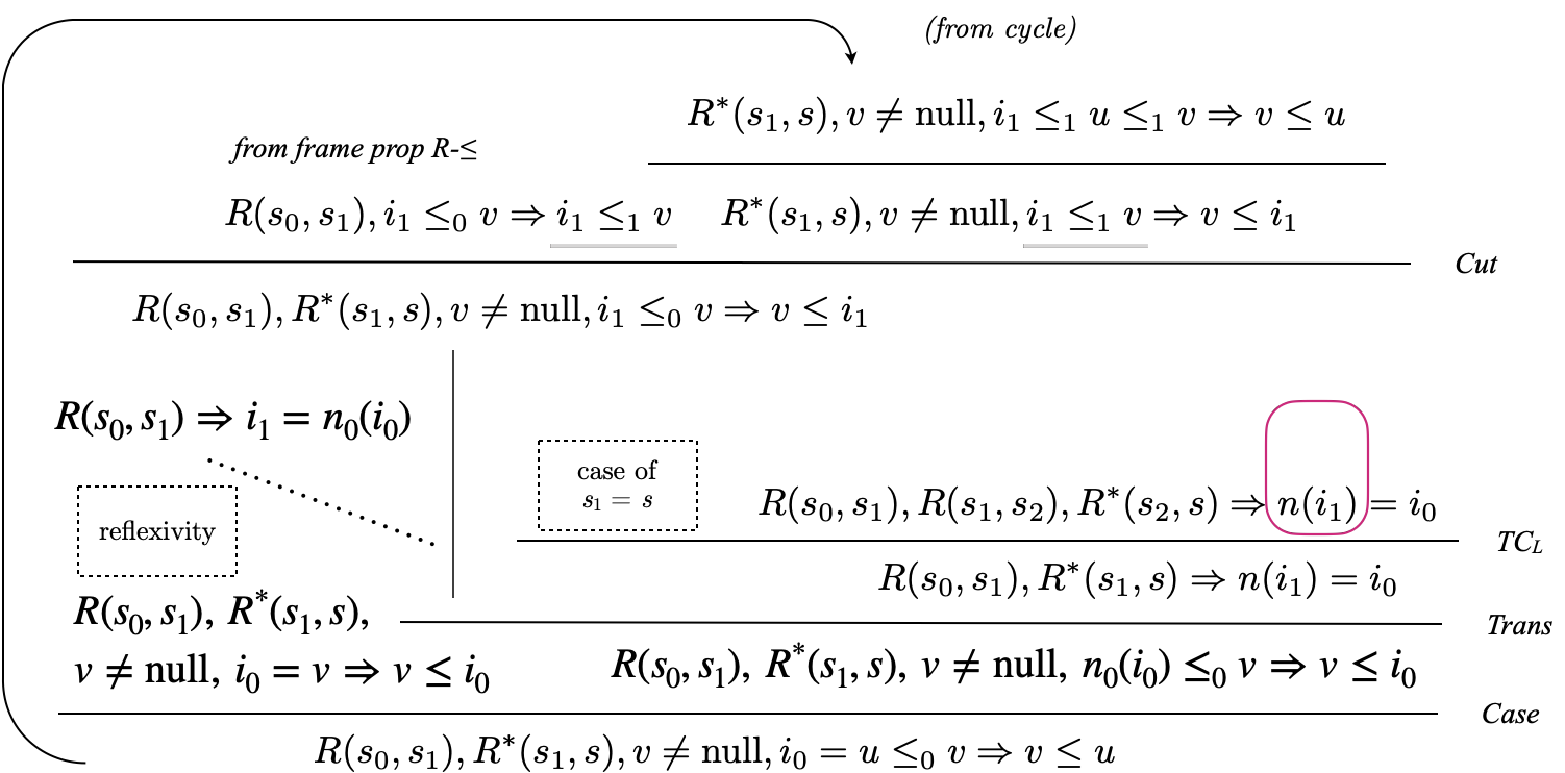
\includegraphics[width=4.5cm]{img/concept-art-atp.pdf}%
\hspace{-1mm}%
\raisebox{-1.25cm}{
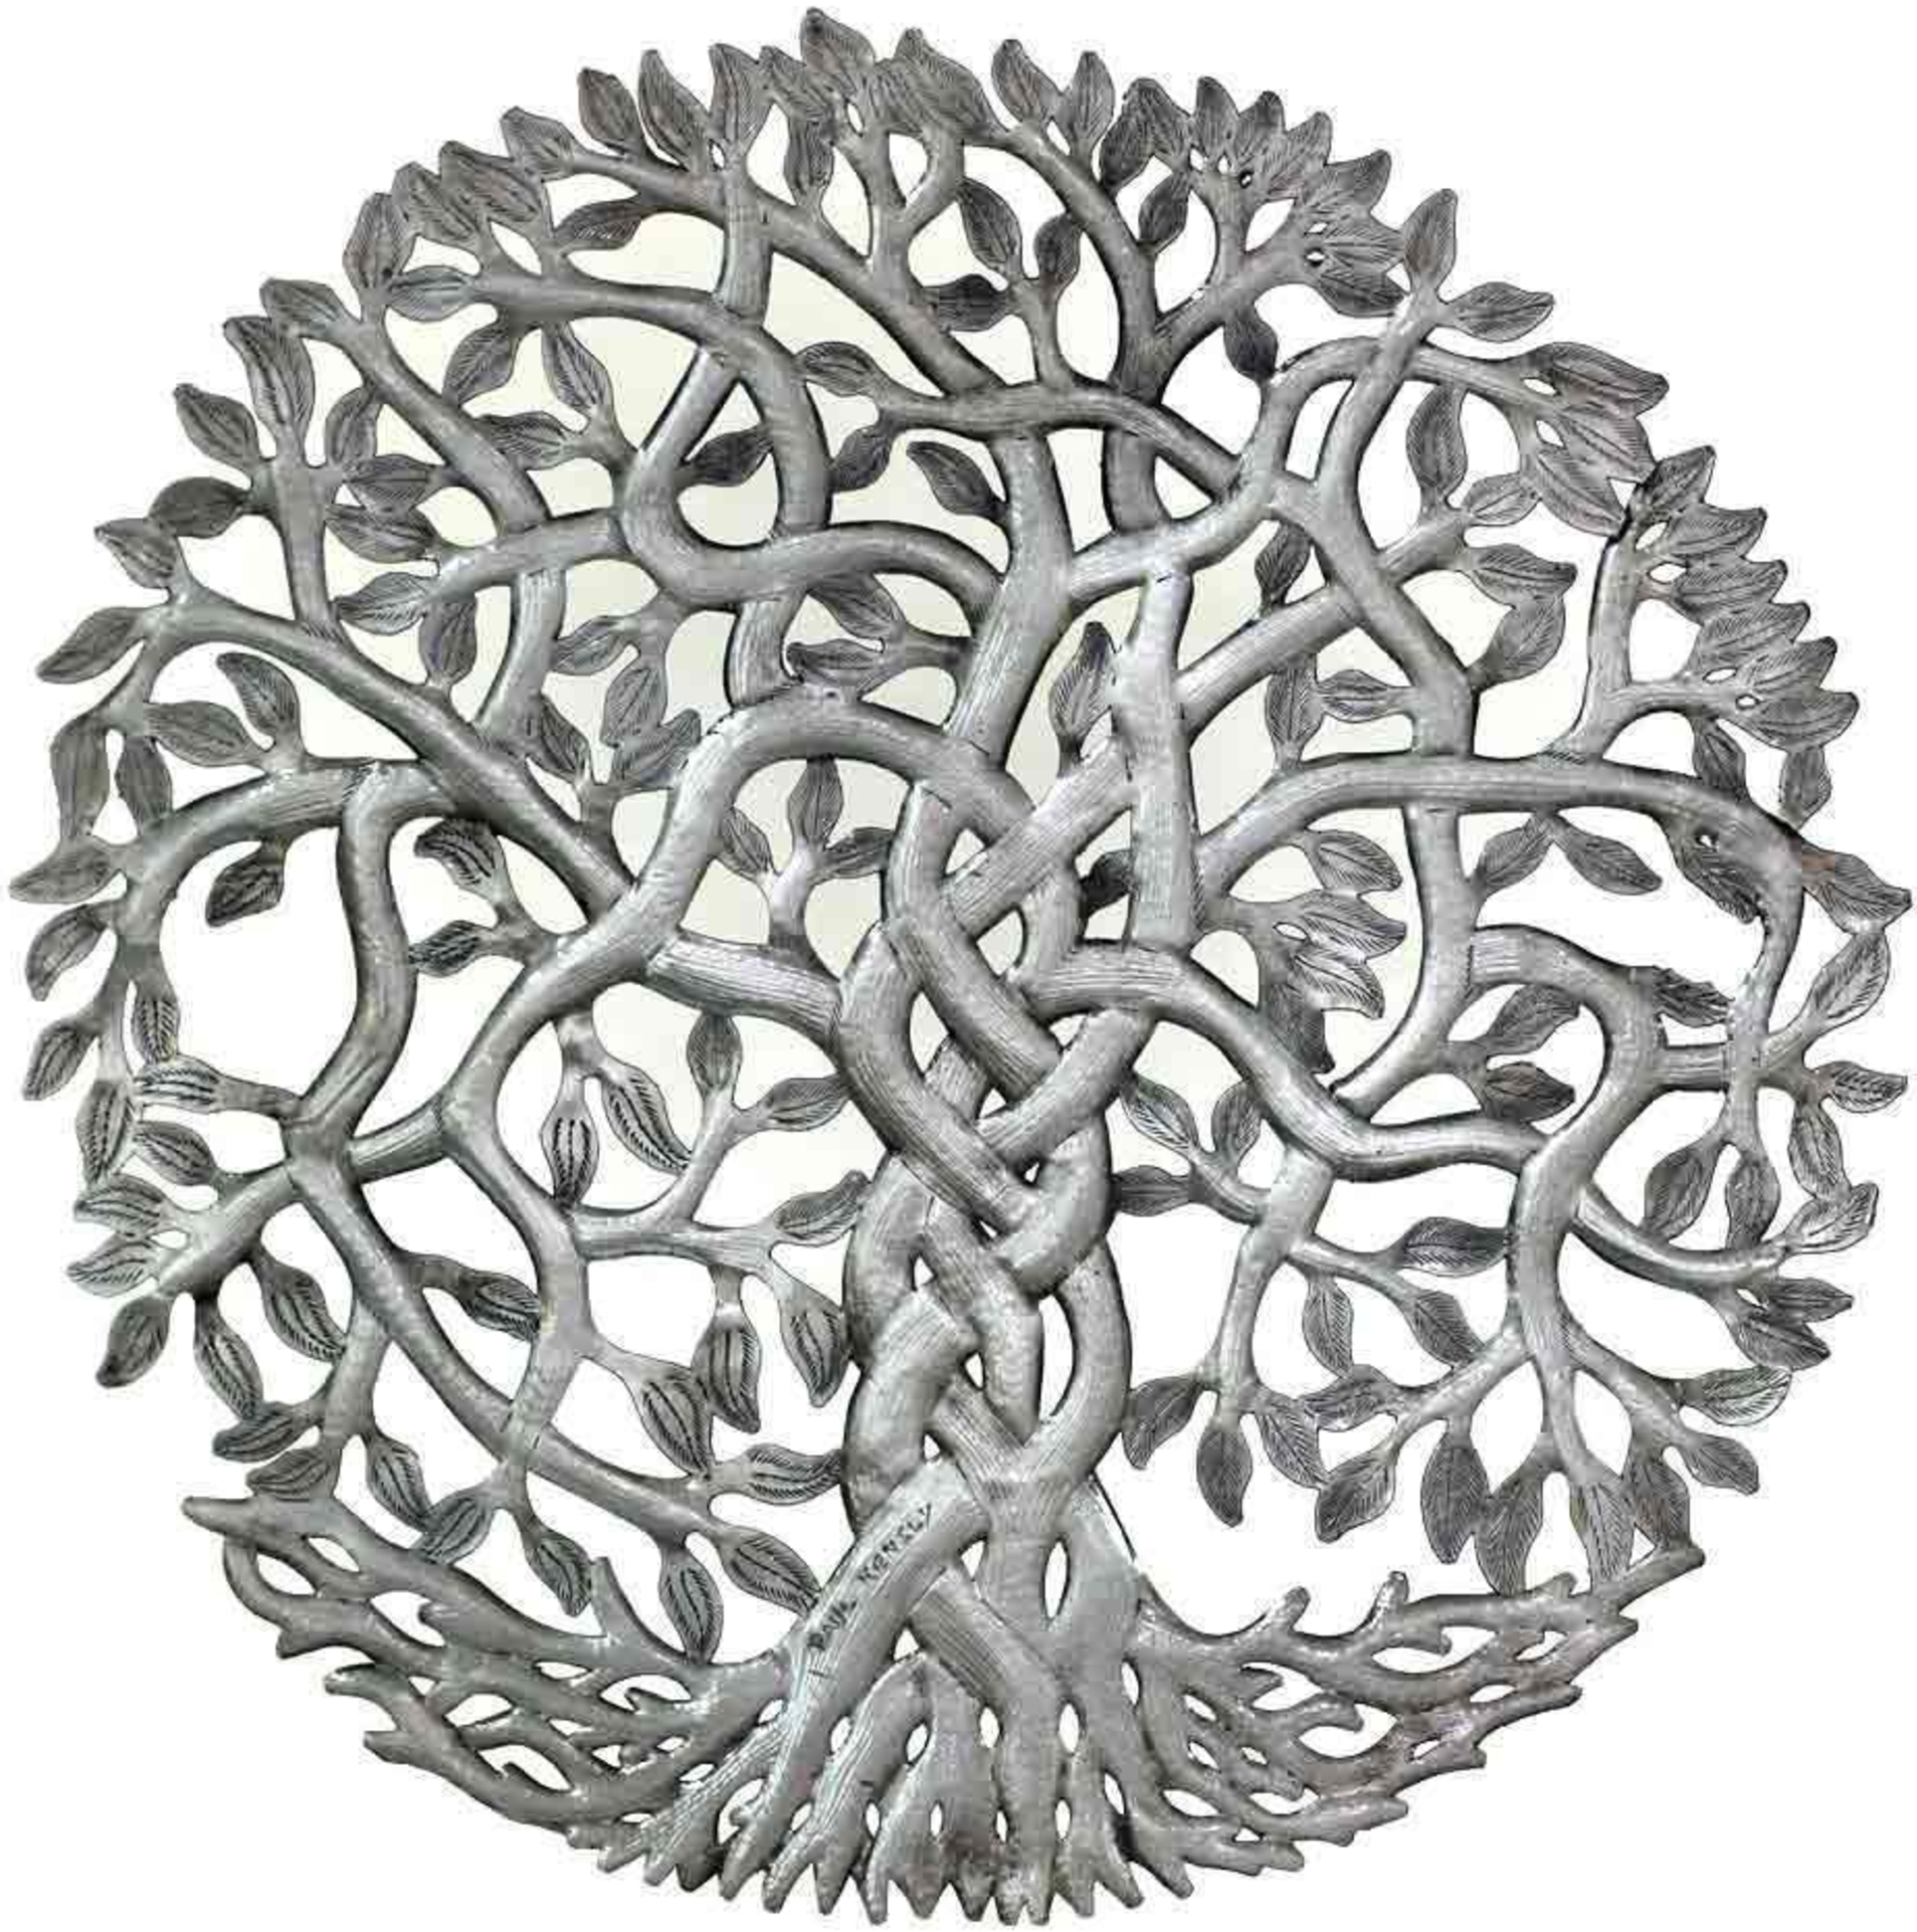
\includegraphics[width=4.5cm]{img/entangled-tree-of-life.pdf}%
}%
\hspace{-9pt}%
\raisebox{5mm}{
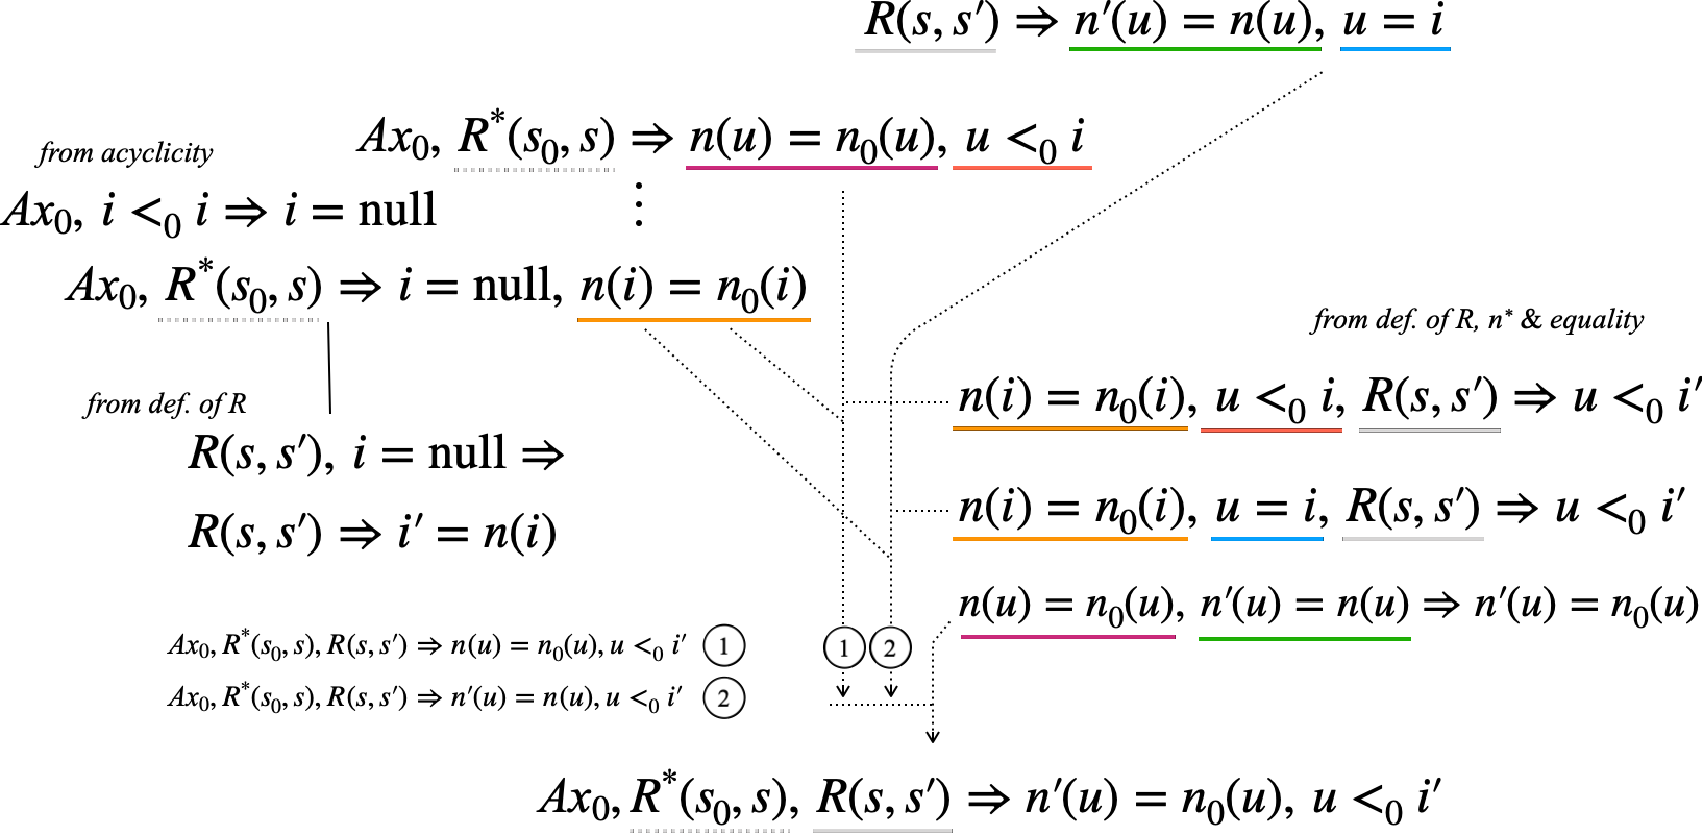
\includegraphics[width=4.5cm]{img/concept-art-smt.pdf}}
\end{center}


\clearpage

\section*{Satisfiability Modulo Theories and Automated Theorem Proving:\\ Quest for the Missing Link}

\vspace{-.5em}
\hrule

\vspace{1.2em}
Beginning with the 1980's, the computer science community has accepted
that computer programs and logical proofs are made of the same fabric.
They are both based on a rigorous formal language, characterized by a grammar,
and they both rely heavily on tree-like structures for defining their semantics,
via syntax-directed derivations.
By now, it has become widely accepted~\cite{curry-howard} that the task of writing a program can be
reduced to that of finding a proof to a conjecture, and conversely, the task of
proving a theorem can be reduced to producing a program with some specific
characteristics.
In addition to that, logic is at the core of software verification, as a basis
for specifications~\cite{dafny,boogie,seahorn}, loop invariants~\cite{ic3,spacer,..}, rely-guarantee properties~\cite{relyguarantee1,..}, and more.
The task of checking adherence to a program's specification is also reduced, in
more than one way, to deciding the validity of a logical formula.

\medskip
This proposal is based on a fundamental understanding, that breaking existing
barriers in automated reasoning is a key ingredient that will lead to
much more powerful mechanism for the construction of provably-correct software.
By powerful, we mean scalable to the sizes of realistic software modules,
adaptable to arbitrarily complex properties,
and requiring less user effort thanks to an increased level of automation.
To achieve this goal, this research \textbf{aims to bridge the gap between two insofar prevalent automated  reasoning disciplines}:

\begin{paragraph}{Automated Theorem Provers (ATP)} A family of tools and techniques based on proof
theory of logical deduction.
A logic in this setting is characterized by a vocabulary and a system of
inference rules; provers are tasked with searching the space of proofs, which
are essentially trees (more generally, DAGs) constructed from repeated
application of the inference rules.
\end{paragraph}

\begin{paragraph}{Satisfiability-Modulo-Theory Solvers (SMT)} A somewhat newer approach with roots in complexity theory and algorithms for solving the Boolean satisfiability problem (SAT).
These algorithms have been augmented with decision procedures for several first-order fragments.
SMT solvers have become incredibly popular thanks to highly efficient implementations and very successful optimization heuristics that manage to combat the inherent intractability of the problem.
\end{paragraph}

\medskip

%\todo{Merge description of ATP and SMT to the background; write here a short paragraph defining these two things and saying that the idea is to merge them}


%The expected result is a proof leading to a desired statement (closed formula)
%$\varphi$, that can be used as a certificate to the logical validity of
%$\varphi$ --- that is, it can be checked mechanically to confirm the soundness
%of each inference step.
%While proof search can be a very costly process, due to the inherent complexity
%of the search space, checking a proof is usually swift and done with linear
%cost with respect to its size.

\begin{comment}

%\begin{comment}
\todo{remove this from here and put in background, it kills the flow}
It is worth mentioning a third camp, that has, so far, received less
attention from the programming languages and automated reasoning crowd.

\paragraph{CSP Solvers} Constraint Satisfaction Problems (CSP) are ubiquitous
in planning, AI, and various other fields of computer science.
The ultimate goal of CSP is to find parameters that satisfy a set of (mostly
numerical) constraints. The solutions can be useful for scheduling tasks,
motion planning, \etc.
CSP solvers excel at solving puzzles such as the $N$-queen problem or Sudoku.
Their use in automated theorem proving is insofar limited.
\end{comment}

\medskip
These two camps, coming from such different backgrounds,
face a serious gap,
one that currently prevents adoption of results from one approach into use in
the other.
The primary goal of this research is to construct a unified framework for automated reasoning, where proving
and solving techniques can cooperate.
Such framework need not be constrained by the boundaries of some specific logic, such as first-order logic or linear integer arithmetic.
Instead, careful parameterization will allow adaptive treatment of a wide spectrum of domains, where existing techniques can be seen as individual points in the more general space.
This will allow to leverage the power of ATP and SMT into proving the more complex
conjectures required for software verification and synthesis.
When it comes to applying SMT, one major obstacle in many problem domains, is
that SMT solvers are generally restricted to first-order logic; at the same time,
the properties one wishes to prove require reasoning about composite structures (such as lists, maps, and streams), and, most often, the use of induction.
Theorem provers can more easily be equipped with higher-order logic and induction-oriented inference
rules.
Still, sub-problems arising in the course of resolving the induction step can
and should benefit from honed SAT and SMT capabilities.

As an overarching goal, this research will \textbf{lay foundations for a new discipline
in automated provers, by way of integrating the camps of ATP and SMT and allowing
cross-fertilization}.
Specifically, it is motivated by provers for the tasks of software verification
and synthesis; these are characterized by relying almost exclusively on discrete
mathematics, such as set theory, graphs, automata, an algebraic construction of
natural numbers, and various theories of integer arithmetic.


\section{Background}

%\todo{The background should put an emphasis on what each tool is good at}

\begin{paragraph}{Automated Theorem Provers}
Proof theory is a branch of logic that has gained much traction in the 20th century with the advent of Hilbert~\cite{Book1928:Hilbert} and Gentzen~\cite{j1935:Gentzen},
both of whom developed calcli for algorithmic formalization of proofs.
As computers became available, it was natural that these notions be implemented as programs.
As early as 1960~\cite{otter}, large automatic systems for theorem provers have been used by the research community for a variety of logical reasoning tasks.
Most of these early systems were based on the resolution principle~\cite{robinson1965}, which continues to be popular today.
Term unification~\cite{robinson1965} is used to resolve first-order formulas.
In the 1990's, superposition calculus~\cite{LPAR1992:Bachmair} emerged as the leading technique for equality reasoning.
This led to several successful theorem provers, notably Vampire~\cite{JAR1995:Voronkov} and E prover~\cite{AIC2002:Schulz}.
Today, most theorem provers rely in one way or another on term rewriting for the implementation of superposition, based on the Knuth-Bendix algorithm~\cite{knuth-bendix} for normalizing rewrites.

More recently, a lot of attention was directed towards \emph{cyclic proof systems}, a form of Gentzen-style calculus that natively admits proof by induction.
Instead of the traditional induction scheme or induction rule, \eg (for $\mathbb{N}$) $P(0)\land \forall k.\,P(k)\to P(k+1) \vdash \forall n.\,P(n)$,
cyclic proofs admit ancestor sequents as premises to a later inference steps --- thereby allowing the proofs to contain cycles.
To avoid unsoundness caused by a self-referencing statement, cyclic proof systems impose a \emph{global trace condition} that ensure cycles cannot be unrolled \textit{ad infinitum}.
This trace condition is carefully crafted for every cyclic system to enable a soundness proof for the system.
In a way, whatever complexity is removed from the proof proper is shifted to the global trace condition;
however, this allows for some pretty sophisticated trace conditions, such as those based on B\"uchi automata.
In turn, these allow such systems to provide exetremely succinct and elegant proofs.
\end{paragraph}

\begin{paragraph}{Satisfiability-Modulo-Theory Solvers}
A somewhat newer approach based on extending the
Boolean satisfiability problem (SAT) with first-order theories and arithmetic, leading to
Satisfiability Modulo Theory (SMT).
SAT solvers accept Boolean formulas and construct a satisfying assignment, or
declare that none exists.
Since SAT is NP-complete (in fact, usually referred to as \emph{the} canonical
NP-complete problem), finding the solution may be time consuming, but eventual
termination is guaranteed.
SMT solvers take first-order formulas and attempt to find a first-order
\emph{model} for them, that is consistent with an underlying theory --- where the
theory is built into the solver.
The theories generally put no bound on the size of the models they admit
(\eg, numerical theories are typically defined over the domain of integers),
and as expected, the problem is generally undecidable.
However, despite the inherent complexity of SAT and undecidability of SMT,
solver technology has become extremely successful, especially in applications
relating to software verification.
In this context, proving a verification condition (``theorem'') $\varphi$
amounts to finding its negation $\lnot\varphi$ unsatisfiable --- which is the root
of the connection, and contention, between SMT solvers and theorem provers.
For many software verification conditions, SMT solvers have been shown to be
more effective in proving the validity of verification conditions than
contemporary proof theory-based theorem provers.

SAT and SMT received much tractions in the Model Checking community~\cite{clarke-grumberg} thanks to their successful applications to formal methods.
SAT was initially utilized for hardware verification of logical circuits, and SMT became a natural extension for dealing with software, as programming languages typically provide primitives such as integer values~\cite{CAV2006:Dutertre}, bit vectors~\cite{TACAS2007:Bryant}, and arrays~\cite{CAV2007:Ganesh}.
Because loops are pervasive in both hardware and software systems, there is an ever-present need for reasoning about executions of unbounded length.
To that end, \emph{loop invariants} play a crucial role in all software verification systems~\cite{dafny,fstar,leon}.
This essentially facilitates an induction scheme, but, by and large, the burden of supplying the invariant remains with the programmer.
\emph{Invariant inference} is a big open problem that stands in the way to effective software verification.
A significant breakthrough in invariant inference was achieved last decade with the development of the IC3 algorithm~\cite{bradley11} for automatic inference of Boolean invariants for hardware model checking.
This sprouted a line of successful follow-up works on Property-Directed Reachability~\cite{gurfinkel,shoham,vizel}.
These results have been integrated into the leading SMT solver Z3~\cite{z3,spacer} and form key components of the SeaHorn verifier~\cite{seahorn} for C programs.
\end{paragraph}


\section{Bridging the Automated Reasoning Gap}

%\todo{Be more specific about the problems and why they are important: e.g. "cope with Boolean constructs", "unavoidable in software verification" etc.; explain what gives rise to these instances}

\begin{paragraph}{Objective 1: {\it Bridging equality and congruence}}~
Equality and equivalence are fundamental terms in mathematics and computer science.
Therefore, equality is a native primitive in most logics.
SMT solvers rely on a decision procedure for (quantifier-free) congruence closure together with the Nelson-Oppen method for combining it with other theories.
ATPs, by and large, are invested in superposition calculus, which is driven by term rewriting.
To support efficient rewriting and avoid backtracking, modern ATPs such as Vampire and E employ an order relation on terms, so that all rewrites are directed.
Both of these approaches limit the provers' ability to reason about equalities given as assumptions or discovered as conjectures in the course of the search:
This is due to the quantifier-free nature of Nelson-Oppen, leading to a constant need for speculative quantifier instantiation, on one hand;
and the requirement for ordering, which relies on the Knuth-Bendix algorithm, which in turn is incomplete --- so it cannot be expected to produce a normalizing ordering for an arbitrary set of univerally-quantified equalities that has been accumulated.
We propose, as a unifying mechanism, to further utilize the notion of \emph{equality graphs} (e-graphs), as is done in some SMT solvers~\citeneeded{} for performance purposes.
We combine this with term rewriting and \emph{equality saturation} to obtain \emph{unordered} sets of equivalence terms (e-classes).
E-graphs are known to be space-efficient by reducing duplication in the representation of terms to a minimum, employing congruence closure as a core mechanism to merge class nodes and keep the graph compact.
This knowledge is maintained as part of the prover's state and can be updated incrementally when the prover discovers new conjectures.
To cope with Boolean constructs (such as implications and disjunctions, which are frequent in verification conditions due to the presence of branching statements in programs), we propose a novel solution, \emph{e-graph coloring}, by which sub-components of the e-graph can be annotated with certain ``colors''; the colors denote that the validity of some propositions is subject to one or more assumptions, in the spirit of Gentzen's sequents.
This enables the use of assumptions similar to how they are introduced in CDCL(T), with easy backtracking when a conflict occurs.

This will lay a foundation in which e-graphs are the glue that binds SMT-style equality reasoning, that is based on congruence, and the ATP-style superposition, without requiring terms to have a normal form, and while incorporating the power of SAT in handling Boolean conditions and predicates.
\end{paragraph}

\begin{paragraph}{Objective 2: {\it Bridging induction}}~
The success of SMT solvers with first-order reasoning led to their wide adoption in software verification.
This gives rise to the challenge of representing unbounded state (\eg size of data structures) and unbounded time (\eg number of loop iterations).
The proposed framework will try to generalize and unify the two leading frontiers for reasoning by induction.
In the world of model checking and SMT, the IC3 algorithm and its variants~\todo{remember to cite them in the background} has proven to be the gold standard for automatic invariant inference.
In proof theory and deductive reasoning, cyclic proof systems provide shorter proofs, which have good value for ATPs such as Cyclist, where proof search is severely limited by the depth of the proofs that can be feasibly explored.
These two approaches to proof by induction are vastly different: IC3 is counterexample-driven; Cyclist is proof-driven.
We plan to draw on the duality between reachability and invariant inference~\citeneeded{padon} to create a unified description of the two processes, where both aspects, inductive and deductive, will manifest.
This new setting would allow the conclusions accumulated with the IC3 method to direct and guide the proof search, and intermediate conclusions from closed cycles in the pre-proof being constructed to inform the clause inference that is a core step of IC3.

More broadly, IC3 can be seen as a process where a proposition is repeatedly \emph{strengthened} until it becomes inductive and can be used as an inductive loop invariant.
Constructing a proof can also be seen as starting with a proof goal and strengthening it by choosing (a set of) subgoals that entail it.
On the other hand, both processes have crucial elements of \emph{weakening} as well: in IC3, a single counterexample (represented as a \emph{cube}, \ie, a conjunction of literals) needs to be generalized in order to ``block'' an entire set of unreachable states.
This is essential to IC3's good performance relative to more traditional model checking.
In deductive proof search, \emph{cuts} are required to support the construction of proofs by case analysis.
Each case represents a conjecture that is weaker than the general proposition, and knowing which  cases to create is known to be a pain point in automated deduction.
We plan to use partial solutions from over-approximation of the set of reachable ``states'' (representing logical structures) to assist in pruning a deductive proof search process and as a way to suggest conjectures that can be used in case analysis.
Conversely, sequents inferred during proof search can be used in generalizing counterexamples as part of the ``block'' phase of IC3, leading to more effective generalizations and better convergence properties.

To allow seamless information exchange between these frameworks, we propose a method for putting them on a common mathematical foundation.
We draw inspiration from~\cite{Book2003:Avron}, where it was shown that all instances of finitary induction, \ie, induction over countable domains, can be captured by FO(TC) --- first-order logic extended with \emph{transitive closure}.
TC provides a good middle ground for combining induction strategies because
(i) it naturally captures the notion of reachability around which IC3 is built, and
(ii) it has been successfully formulated within the cyclic proof framework~\citeneeded{liron-tc-cyclic}.
Moreover, the latter also facilitates coinduction, which allows proofs over infinite traces (\ie, non-terminating executions).
This may give rise to a new adaptation of IC3 to coinduction, which has not been proposed until now.

State-of-the-art software verification tools such as Spacer employ an intermediate representation of the verification task as a system of Constrained Horn Clauses (CHCs)\todo{make sure these are mentioned in the background} and apply IC3 in order to solve them.
An interesting problem in CHC solving arises when clauses are \emph{non-linear}, that is, the body (left-hand side of the implication) of the rule contains more than one uninterpreted literal.
A similar problem arises in reasoning with TC logic when trees (rather than chains, or sequences) are involved.
Both require handling \emph{branching} paths during exploration.
Combining partial results from both disciplines will provide a more complete solution to this problem,
and improve our understanding and treatment of branching induction in proofs.

\todo{say here: IC3 is good at finding invariants and the like, cyclic proofs are good at [other things], therefore...}

%\todo{IC3 is counterexample-driven; Cyclist is proof-driven. We plan to draw on the metioned duality to construct a tool that maintains and over- and under-approximation of the space of states/logical structures}
%\todo{use a generalized framework: - use cyclic proof search to locally block counterexamples; - use discovered clauses and/or models to prune some branches early, or, conversely, strengthen some hypotheses to make them inductive based on the relative inductiveness of clauses in IC3 frames}
\end{paragraph}


\begin{paragraph}{Objective 3: {\it Combining proof techniques through modular reasoning}}
For an automated reasoning task of any scale beyond trivial, decomposing goals into sub-goals that can be solved independently is an invaluable tool.
This is especially true when it comes to software verification, and the need for it is only emphasized by broadening the scope of acceptable logics and theories.
Putting in mind that a unified framework for automated reasoning strives to combine together proof strategies of several existing tools,
it is even more challenging --- but also potentially more beneficial --- to ``divide and conquer''.
This would increase the flexibility in applying different strategies and automatically turning some exploration features on or off, selectively.
It provides one way of mitigating the risk involved in a more expressive proof system, allowing to take bolder decisions for inclusion of certain inference tactics.

\begin{wrapfigure}[8]{r}{4cm}
\vspace{-1em}
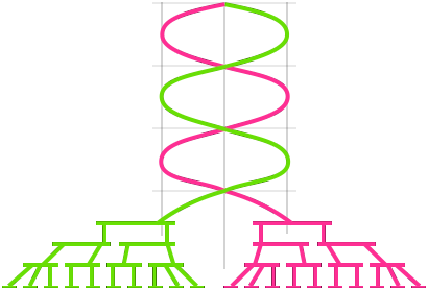
\includegraphics[width=4.5cm]{img/untangled}
\end{wrapfigure}

In a traditional top-down proof search based on a system of inference rules, the prover must reach the system's \emph{axioms} --- rules with no logical premises ---
in order to seal off a proof branch.
Only following successful closure of all proof branches can the prover declare victory.
Two major factors contribute to search-space explosion:
the proof \emph{width}, caused by having multiple rules be applicable at any given point in the proof;
and proof \emph{depth}, caused by the long chain of rules that have to be applied, consecutively, in order to reach the axioms from the proof goal.

%\todo{The key ingredient here is that when searching top-down, you need to reach axioms in the leaves; when combining bottom-up, you can stop earlier when you have reached a lemma that was discovered previously.
%More importantly, the lemma can be discovered by a variety of proof techniques, which can be SMT- or ATP-driven.}
Our modularization approach for more effective theorem proving is based on the introduction and use of \emph{ancillary lemmas}, encapsulating some details of the proof and reducing the search depth by providing a wider range of known facts that can be used as leaves.
Such lemmas are typical in mathematical pen-and-paper proofs, and they are layered on top of one another to be able to convey a complex development.
To amplify the significance of lemmas we propose a novel approach to problem decomposition, called \textbf{untangle-and-conquer}.
As the name suggests, it consists of two phases, the first of which is aimed at splitting a proof goal such that each sub-proof can be comfortably completed using an existing database of lemmas.
We identify the following gap: logical propositions occurring as proof goals contain a mixture of logical symbols from different theories.
For example, they may contain operations on arrays as well as linear arithmetic over the indices and pointer operations on the elements.
In contrast, lemmas are naturally smaller and involve only a handful of symbols.
This applies to both human-constructed lemmas, because the cognitive load required to deal with intricate interactions between too many different concepts is high;
and to automatically generated lemmas (which we discuss shortly), since large vocabularies incur high resource costs to search through.
It is therefore desirable to engineer the proof in such a way, that each part contains a subset of the symbols occurring in the goal.


Oftentimes, choosing the right lemmas to use as stepping stones is the key insight a mathematician has to come up with.
It would definitely be presumptious to expect an automated reasoning program to replicate this much insight; but there are two key factors working to our advantage when dealing with software-oriented proofs:
(i) Even if some lemmas require ingenuity in their formulation, there is an even larger number of simpler, more ``mundane'' lemmas, and finding those automatically removes tedium from the human user;
(ii) Lemmas used in different proofs are often similar, 
so building a database of discovered lemmas can help the prover in future endeavors;
(iii) By the same argument, using a corpus of previously completed proofs (either human- or machine-generated) can guide the search for lemmas and make use of past results.

We are especially interested in \emph{theory exploration} (or \emph{theory forming}):
Given a library of proven properties, an automated reasoning system can eagerly search for consequences, thereby growing the body of ``knowledge'' at the prover's disposal.
Deductive proof search in ATPs such as Vampire and Cyclist tends to be oriented ``top-down'', that is,
starting from a proof goal, simplifying it further and further until axioms are reached.
The is analoguous to building the proof tree from the root down to the leaves. (Although, graphically, proof trees are commonly depicted with the root at the bottom --- this is nevertheless a top-down approach.)
The availability of synthesis technology \cite{quickspec,thesy} means that we can generate a vast number of lemmas to guide our untangle-based decomposition.
The major risk here is that too many lemmas may incur a high overhead and, moreover, produce too many different ways to decompose a given proof.
We propose to mitigate this by developing a ranking method for discovered lemmas based on their usefulness,
so that our automated reasoning tool can \textbf{learn from experience} and get better over time, using classic statistical inference.
\end{paragraph}

\begin{paragraph}{Objective 4: {\it Extrapolating to Software}}~
The overarching goal of this research is to pave the way for the next generation of theorem proving technology.
The emphasis remains on making tools that allow reasoning about properties of computer programs.
What this means is that an automated prover is required to cope with a high volume of low-level details that interact in unexpected ways.
We would like to take advantage of \textbf{inherent abstraction layers} that already exist in software,
since abstraction is what makes it possible
for human programmers to cope with its ever-growing complexity.
One form of abstraction can be used via the ancillary lemmas described above.
An orthogonal axis is the application of \textbf{semi-automatic refinement} to provide encapsulation for some of the implementation details.
For example, an ordered data structure may be abstracted as a set and a (total or partial) order relation; a multi-threaded process may be abstracted as a sequential one that is behaviorally equivalent.
Choosing the abstraction to use in a refinement proof would, more often than not, require some human intuition, which is why some amount of user interaction will be needed.
Our hope is that with the right abstraction in place,  the automated prover will be able to carry out all or most of the refinement proofs,
showing that the abstraction soundly models the underlying implementation and also inferring system invariants from it --- making this process extremely rewarding.

We will focus on the incorporation of Separation Logic and its modern variants such as Iris~\cite{iris} for modeling a program's memory, \esp in programs that use dynamic allocation or multiple threads with shared state.
In essence, what Separation Logic provides is a refinement that \textbf{correlates the low-level, imperative, mutable semantics of pointer programs with high-level, functional, immutable semantics} that are closer to mathematical definitions.
Establishing the correlation, then leveraging it to prove properties of the underlying program, is a fine example of proof modularization.
The pillars of equality reasoning and proof by induction are both central in this effort.
\end{paragraph}


\begin{comment}
% I am not sure what to do with this
Another obstacle, which hinders both approaches, is the use of quantification
in assumptions and theorems.
One generally wishes to take advantage of the inherent modularity in proving
most kinds of properties, be those mathematical theorems in algebra or combinatorics,
and definitely when it comes to correctness properties of computer programs.
Software is modular by nature, 
It is very much desirable to adopt the same contributing factor to reasoning about
these programs.
This means that instead of constructing one monolithic proof of the ``ultimate
theorem'', one identifies and proves \emph{lemmas} that abstract and generalize
domain knowledge and understanding of the underlying program --- layering them
up until the final goal is met.
This is definitely how it is done in academic papers, and, more recently, in
large software verification projects.
Going back to the challenge at hand, these auxiliary lemmas typically include
quantified formulas, which are logic's way of expressing generalized conjectures.
Applying these lemmas, \eg in the context of carrying out the next step of the proof,
ultimately requires to instantiate universal quantifiers with logical terms.
Since the space of available terms is large (or even infinite), this becomes
a task that is daunting to automate and requires the employment of heuristics
to select the right instances.
We will move to consolidate instantiation strategies into ones that more closely
matches the search for proof --- thus being goal-directed rather then origin-directed.
A primary aim is to make these strategies less heuristic and more predictable.
\end{comment}


\section{Risk assessment and expected significance}

My earlier work~\cite{phd} and some follow-up by others~\cite{padon,feldman} revolved around the use of decidable logics to encode verification conditions for software,
and transferring these to an SMT solver.
These decidable fragments are extremely limited, and once you ``cross the line'' of undecidability, performance is largly unpredictable.
There are many practical solvers that are able to prove many naturally occurring problems with arithmetic, arrays, and lists;
but pile up too many undecidable particles on top of one another, and frequent divergence ensues, with little to no recourse for debugging the cause.

The Matryoshka project~\cite{what} set as their target enriching SMT solvers with higher-order constructs such as recursive definitions and second-order quantification.
This allows for a more natural, straightforward encoding of software-related queries, but there is very much a glass ceiling imposed by the SMT core.
This project's aim is to inspire a \textbf{paradigm shift} in prover design, putting less focus on finely-tuned heuristics to cover an ever-increasing set of benchmarks, and diverting more effort to \emph{transparency and comprehensibility} of the results.
Generating short, readable proofs, as well as interpretable explanations in cases of failure to find a proof,
are key to mitigate of the risks and remove of the element of dread that accompanies usage of contemprary ATPs and SMT solvers.
In addition, careful regression experiments that will ensure that our team will not have to reinvent existing technology, but build on the vast experience of the past decades of research.

\clearpage
\hrule
\smallskip
{\centering \small Part B2 starts here

}
\section{State of the art and objectives}

The correctness of computer-controlled systems is an open problem in computer science that, despite significant theoretical advances, does not have a satisfactory, practical solution.
Software has been growing steadily in volume and complexity since the 1970's, and compiler architecture grew along with it.
Automated verification is lagging behind: It has only become reasonably tractable in the early 2000's, at which time the size of software systems was already measured in millions of lines of code.
Since then, it is struggling to catch up with the software industry, while at the same time, technological advances increase our reliance on software as well as the complexity of computer systems.
Most of the quality assurance processes rely on intensive testing, and Symbolic Execution~\cite{symex30years} has become a valuable tool for automatic generation of tests for detecting bugs.
However, such tools do not provide guarantees and cannot prove correctness properties of the underlying program.

All software verification tools follow a common pattern:
First, a frontend inspects the source code and constructs a semantic representation (some examples for this intermediate representation are Boogie~\cite{boogie}, Viper~\cite{viper}, and LLVM IR).
Then, a backend derives a set of \emph{verification conditions} --- logical statements whose validity implies the correctness of the property being verified.
These logical statements are sent to a prover to establish their validity.
This proposal focuses on the latter phase, that of finding the proof of validity, where the input formula is a given.
Still, it is important to remember, that better provers influence the design choices in the upper layers, which may contribute to the overall success of the tool.

\subsection{Recent advances in proof theory}

Automated theorem provers are based on the foundation of formal proof systems.
A proof system consists of a language of \emph{judgements} and a set of \emph{inference rules} that facilitate derivation of new judgements from existing ones.
The most notable proof systems today are a form of \emph{sequent calculus}, where judgements are \emph{sequents} of the form $\Gamma \vdash \Delta$ where $\Gamma,\Delta \subset \Lang$ are finite sets of formulas from a logic $\Lang$, which can be, for example, first-order logic over some vocabulary.
The semantics of $\Gamma\vdash\Delta$ is: for every structure $M$ and valuation $\sigma$, if $M,\sigma\models\varphi$ for every $\varphi\in\Gamma$, then there exists $\psi\in\Delta$ such that $M,\sigma\models\psi$.
The connection with the logical semantics is utilized in meta-proofs about the soundness and/or completeness of the proof system,
but when constructing proofs (manually or automatically) the semantics is largely ignored, and only the syntactic form of the judgement, as embodied in the system's inference rules,
is utilized for reasoning.

\begin{figure}
\centering
\renewcommand\arraystretch{1.2}
\[
\begin{array}{c@{\qquad}c}
\begin{array}{c}
~ \\ \hline
\Gamma \vdash \Delta, \RTC{x,y}{\varphi}{s,s}
\end{array}
\,\rulename{TC$_\textrm{refl}$}
%
&
\begin{array}{c}
\Gamma \vdash \Delta, \varphi[s,r] \quad
\Gamma \vdash \Delta, \RTC{x,y}{\varphi}{r,t} \\ \hline
\Gamma \vdash \Delta, \RTC{x,y}{\varphi}{s,t}
\end{array}
\,\rulename{TC$_\textrm{R}$}
\\[5ex]
\multicolumn{2}{c}{
\begin{array}{c}
\Gamma, s = t \vdash \Delta \quad
\Gamma,\varphi[s,z], \RTC{x,y}{\varphi}{z,t} \vdash \Delta \quad
z~\textrm{\small fresh}
\\ \hline
\Gamma,\RTC{x,y}{\varphi}{s,t}
	\vdash \Delta
\end{array}
\,\rulename{TC$_\textrm{L}$}
}
\end{array}
\]
({\small $\varphi[s,t]$ is a shorthand for $\varphi[s/x,t/y]$})
\caption{An example for a cyclic proof system for transitive closure.}
\label{b2:tc-cyclic}
\end{figure}

Inference rules take the form shown in \autoref{b2:tc-cyclic}: premises are judgements written above the line, and a conclusion is written below the line.
Each rule is, in fact, a \emph{schema}, since the names $\Gamma, \Delta, \varphi, s, t, x$ \etc are placeholders for formulas, terms, or variables, as appropriate.
A proof of a sequent $\Gamma\vdash\Delta$ is, at its core, a sequence $\Phi_1, \Phi_2, {\cdots}, \Phi_n$ of judgements such that each $\Phi_i$ is \emph{derived} from $\Phi_{r_1}, {\cdots}, \Phi_{r_k}$ ($r_{1..k} < i$) using one of the inference rules, and $\Phi_n = \Gamma\vdash\Delta$.
Commonly, $\Phi_{1..n}$ are portrayed in a directed tree where the direct children of $\Phi_i$ are the corresponding $\Phi_{r_{1..k}}$ from the derivation.
If some $\Phi_j$ is used as a premise in more than one derivation step,
there are two alternative ways to represent it:
Either duplicate $\Phi_j$ (and all of its descendants) when depicting the proof as a tree, or switch to a DAG representation where each judgement can have any number of parents.

\begin{paragraph}{Superposition theorem provers and saturation}
The term ``superposition'' is used to describe a family of theorem provers that are based on two main principles of deduction: \emph{resolution} and \emph{superposition}.
Both use the core concept of \emph{unification}.
Given two terms $t_1, t_2$, a \emph{unifier} is a (syntactic) substitution $\theta$ such that $t_1\theta = t_2\theta$.
The equality here designates syntactic identity, and $t\theta$ denotes applying a substitution to a term.
A classical result in logic tells us that if two terms have a unifier, then they also have a \emph{most general unifier} (\emph{mgu}):
A substitution $\theta_1$ is considered more general than another $\theta_2$ if the latter can be obtained from the former via sequential composition, $\theta_2 = \theta'\circ\theta_1$.
Following are a few select inference rules based on this concept.

\noindent\vspace{0pt}
\[
\begin{array}{c}
A \lor C_1 \quad \lnot A' \lor C_2 \\ \hline
(C_1 \lor C_2)\theta^{\scriptscriptstyle A}_{\scriptscriptstyle \!A'}
\end{array}
\,\rulename{RES}
\qquad
\begin{array}{c}
l=r \lor C_1 \quad L[s] \lor C_2 \\ \hline
(L[r] \lor C_1 \lor C_2)\theta^{s}_{l}
\end{array}
\,\rulename{SUP$^=_0$}
\qquad
\begin{array}{c}
l=r \lor C_1 \quad t[s]=t' \lor C_2 \\ \hline
(t[r]=t' \lor C_1 \lor C_2)\theta^{s}_{l}
\end{array}
\,\rulename{SUP$^=_1$}
\]

In the above, $\theta^{\alpha}_{\!\beta}$ is the mgu of $\alpha$ and $\beta$.
In addition to that, a superposition inference system makes use of an extra \emph{simplification order} $\succ$ on terms.
In \rulename{SUP$^=_0$} and \rulename{SUP$^=_1$},
application is restricted to cases where
$t'\theta \not\succeq t[s]\theta$.
This breaks the symmetry of equality and provides the prover with a direction.

Vampire~\cite{vampire} is the most reknown superposition theorem prover.
It works by \emph{saturation}: Vampire maintains a set $D$ of first-order clauses,
and incrementally grow it by selecting $\Phi_{r_{1..k}} \subseteq D$ and adding a clause $\Phi_{n+1}$ according to one of the inference rules.
Vampire terminates when it derives the empty clause ($\bot$, representing a contradiction),
or when $D$ is saturated, \ie, no new clauses can be added.
\end{paragraph}

\begin{figure}
\centering
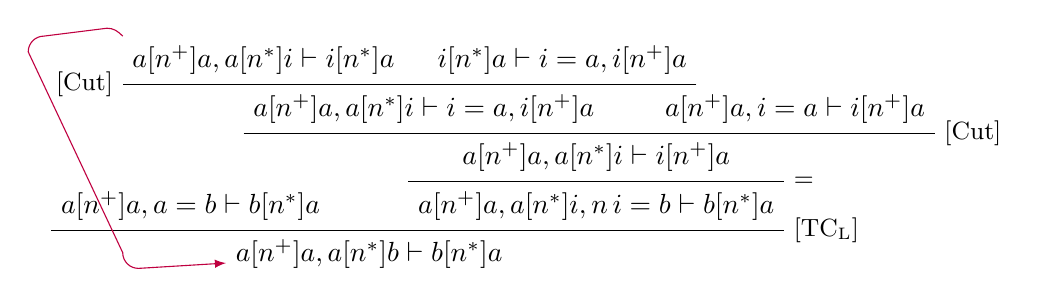
\begin{tikzpicture}[>=latex]
  \node(u0) { $a[n^+]a, a[n^*]b \vdash b[n^*]a$ };

  \node(u1)[above=0 of u0, anchor=south east, 
            xshift=-.5cm] 
  { $a[n^+]a, a=b \vdash b[n^*]a$ };

  \node(u2)[above=0 of u0, anchor=south west,
            xshift=.5cm] 
  { $a[n^+]a,a[n^*]i,n\,i=b \vdash b[n^*]a$ };
  
  \draw (u1.south west) -- (u2.south east)
    node[right] {\small [TC$_{\textrm{L}}$]};

  \node(u3)[above=0 of u2]
  { $a[n^+]a,a[n^*]i \vdash i[n^+]a$ };

  \draw (u2.north west) -- (u2.north east) 
    node[right] {\small =};

  \node(u4)[above=0 of u3, anchor=south west, 
            xshift=.75cm]
  { $a[n^+]a,i=a \vdash i[n^+]a$ };
  \node(u5)[above=0 of u3, anchor=south east,
            xshift=.1cm] 
  { $a[n^+]a,a[n^*]i \vdash i=a, i[n^+]a$ };

  \draw (u5.south west) -- (u4.south east)
    node[right] {\small [Cut]};

  \node(u6)[above=0 of u5, anchor=south west, 
            xshift=.05cm]
  { $i[n^*]a \vdash i=a, i[n^+]a$ };
  \node(u7)[above=0 of u5, anchor=south east, 
            xshift=-.25cm]
   { $a[n^+]a, a[n^*]i \vdash i[n^*]a$ };
   
  \draw (u6.south east) -- (u7.south west)
  	node[left] {\small [Cut]};
      
  \draw[->,purple] (u7.north west) to[out=135,in=0] +(-2mm,+1mm)
    -- +(-1cm,0 ) to[out=180,in=90] +(-1.2,-2mm) 
    -- +(0,-2.75cm) to[out=-90,in=180] +(+2mm,-2.95cm) -- (u0);

\end{tikzpicture}
\caption{An example for a cyclic proof with transitive closure.}
\label{b2:tc-cyclic-example}
\end{figure}

\begin{paragraph}{Cyclic proofs}
Traditionally, proofs are required to be finite, which is a sensible design choice, since the most important aspect of formal proofs is that they can be checked mechanically and validated by an algorithm.
However, more recently, a somewhat surprising player entered the field by challenging this restriction and allowing infinite proofs~\cite{LICS2007:Brotherston}.
Relaxing the finitary condition demands another, external condition in order to preserve the soundness of the proof system.
It is perhaps this \textbf{separation of concerns} that admits cyclic proofs that are more compact and elegant than traditional finitary proofs --- which is what brought them growing popularity.

In the cyclic framework, derivations are permitted to be regular,
non-well-founded (\ie,~infinitely tall) trees.
Regularity ensures that an infinite derivation tree always has a finite representation
as a (possibly) cyclic graph.
Concretely, these derivations are represented as finite trees, 
along with a set of \emph{backlinks} connecting each
non-terminal leaf node --- called \emph{bud} ---
to a syntactically identical ancestor node --- called \emph{companion}.
In other words, we allow goals from the middle of the proof to be
used again as premises higher up the derivation tree.
Formally, each backlink denotes the infinite unfolding of the
path connecting the bud with its associated companion.
We call such derivations \emph{pre-proofs}, since, alluding to the proofs-as-programs duality, they do not necessarily correpond to \emph{terminating} programs.
To ensure termination, we require that pre-proofs satisfy
an additional global property, defined in terms of \emph{traces} of syntactic elements, which can be formulas or terms.

A \emph{trace} is a sequence of formulas $\varphi_1, {\cdots}, \varphi_n$ that appear along a path in the proof tree (not counting the backlinks).
For a cycle consisting of the sequents $\Phi_1,{\cdots},\Phi_n$, where $\Phi_n$ is the bud and $\Phi_1$ is the companion, we define the \emph{trace condition} as follows:
\begin{enumerate}
 \item Each $\varphi_i$ occurs in the corresponding $\Phi_i$.
 \item $\varphi_i \sqsubset \varphi_{i+1}$ for every $i=1..(n-1)$, where $\sqsubset$ is a global (partial) order over formulas.
 \item $\varphi_1 = \varphi_n$ (recall that $\Phi_1 = \Phi_n$ because of the cycle).
\end{enumerate}
\end{paragraph}


\subsection{Recent advances in SAT and SMT}

Interest in algorithms for solving Boolean satisfiability (SAT) began with the development of the DPLL method~\cite{DPLL1,DPLL2}.
In its core it is very simple:
It operates on a propositional CNF formula (conjunction of clauses), and follows two main principles:
(a) the \emph{unit propagation rule}, whereby a clause with a single literal determines the truth value of the variable therein; and
(b) the \emph{pure literal elimination rule}, whereby a variable occurring either only positively or only negatively can be omitted.
Whenever the procedure assigns a value of \emph{true} to some literal, the entire clause containing it is discharged.
When a value of \emph{false} is assigned, the literal is removed from the clause.
This can lead to the rules (a) and (b) being enabled many times in the course of execution.
Of course, (a) and (b) alone are not enough to solve all instances, so some guess-and-backtrack is needed to handle the unassigned variables.
Which values to guess and how to backtrack in a way that maintains the most information is crucial for the performance of the solver.

Conflict-Driven Clause Learning (CDCL)~\cite{CDCL} is the gold standard of SAT solvers today.
CDCL improves over DPLL by using \emph{non chronological} backtracking, allowing the solver to undo several decisions at once, and preserving the information obtained from the failed branch in a \emph{conflict clause} that is added to the collection.
The conflict clause then guides future decisions for assigning truth values to variables.
CDCL solvers such as CaDiCaL~\cite{SAT2020:CaDiCaL} are being actively developed to this very day.
Techniques and heuristics for choosing the backtracking destination and constructing conflict clauses is an active research area.

Despite the complexity of SAT (it is NP-complete), today's solvers are capable of solving surprisingly large instances occurring in hardware verification.
For software verification, propositional logic is much too low-level to comfortably express our properties and semantics.
The research community was able to leverage the success of SAT solvers and extend it to satisfiability of first-order formulas, leading to Satisfiability Modulo Theories (SMT).
The ``theories'' refer to specific fragments of first-order logic for which efficient decision procedures have been constructed.
These theory solvers are then composed with the underlying SAT procedure to handle logical connectives.
The combined method is referred to CDCL(T) (previously, DPLL(T)).

\begin{SCfigure}
\begin{tikzpicture}[>=latex,
	buzz/.style={decorate,
    decoration={snake, amplitude=1pt,
      segment length=5pt}}, baseline=(s4.center)]
      
  \node(fol)
  { $g(a)=c \land \big(f(g(a))\neq f(c)
    \lor g(a)=d\big) \land c\neq d$ };
    
  \node(prop)[below=of fol]
  { $A \land (\lnot B \lor C) \land \lnot D$ };
  
  \node(sat1)[right=of prop, draw]
  { \small
    $\begin{array}{cccc}
        A  &  B  &  C  &  D  \\
      \top & \bot & \bot & \bot \\[-2pt]
     \end{array}$ }; 
      
  \node(uf1)[below=0 of sat1]
  { \small
    $\begin{array}{r@{~}c@{~}l}
       g(a) &=& c \\
       f(g(a)) &\neq& f(c) \\
       g(a) &\neq& d \\
       c &\neq& d
     \end{array}$ };
      
  \node(conflict-uf1)[below=0 of uf1, xshift=-1.25cm]
  { $g(a)=c \to f(g(a))=f(c)$ };
  
  \node(conflict-prop1)[below=of prop]
  { $(\lnot A \lor B)$ };
  
  \node(sat2)[left=of conflict-prop1, draw]
  { \small
    $\begin{array}{cccc}
        A  &  B  &  C  &  D  \\
      \top & \top & \top & \bot \\[-2pt]
     \end{array}$ }; 

  \node(uf2)[below=0 of sat2]
  { \small
    $\begin{array}{r@{~}c@{~}l}
       g(a) &=& c \\
       f(g(a)) &=& f(c) \\
       g(a) &=& d \\
       c &\neq& d
     \end{array}$ };
     
  \node(conflict-prop2)[below=1.5 of conflict-prop1,
  	inner ysep=1pt]
  { $(\lnot A \lor \lnot C \lor D)$ };
  
  \node(unsat)[right=of conflict-prop2,draw] { UNSAT };

  \draw[->] (fol) -- (prop);
  \draw[buzz] (prop) -- ($(sat1.west) - (2mm,0)$)
  	node[coordinate](i){};
  \draw[->] (i) -- +(1mm,0);
  \draw[dashed] (prop) -- node[left]{$\land$} 
                (conflict-prop1);
  \draw[->] ($(uf1) - (8mm,2mm)$) -- (conflict-uf1);
  \draw[->] (conflict-uf1) -- (conflict-prop1);

  \draw[buzz] (conflict-prop1) -- 
              ($(sat2.east) + (2mm,0)$)
  	node[coordinate](i){};
  \draw[->] (i) -- +(-1mm,0);
  \draw[dashed] (conflict-prop1) -- node[left]{$\land$} 
                (conflict-prop2);

  \draw[->] ($(uf2) + (9mm,-1mm)$) -- (conflict-prop2);

  \draw[buzz] (conflict-prop2) -- 
              ($(unsat.west) - (2mm,0)$)
  	node[coordinate](i){};
  \draw[->] (i) -- +(1mm,0);

\end{tikzpicture}
\caption{Demonstration of an SMT procedure, outlining the dialogue between the propositional SAT solver and the theory solver (in this case, QFUF --- quantifier-free uninterpreted functions).}
\end{SCfigure}

\section{Research Plan \todo{B2}}


\subsection{Bridging equality reasoning}

Equality is a fundamental concept in mathematics.
The most basic algebraic structures, such as groups,
are models (in the logical sense) of a set of equational
axioms, the likeness of $x\cdot(y\cdot z) = (x\cdot y)\cdot z$ and $x\cdot 1 = 1\cdot x = x$.
Equality is crucial for automated reasoning, because it means that mathematical objects can have more than one name --- multiple terms may represent the same object.
An inference rule $\infruleshort{K}{P(x),Q(x)}{R(x, x+1)}$
can be applied to derive a goal such as $R(y+z, y+z+1)$,
by instantiating $x\mapsto y+z$;
but it cannot be applied directly to a goal such as
$R(y+1, y+2)$, because it does not (syntactically) match the conclusion pattern $R(x,x+1)$.
The goal first has to be rephrased as the two subgoals
$y + 2 = (y + 1) + 1, R(y+1, (y+1)+1)$, using the so-called \emph{paramodulation} rule%
~\cite{Book2001:Nieuwenhuis},
at which point $K$ can be applied to the second subgoal.
The first subgoal is proved independently using an appropriate axiomatization of the integers.

The paramodulation rule is powerful as it allows the prover to subsitute any term $t_1$ with any other term $t_2$, provided that it can then prove the conjecture $t_1 = t_2$.
This is an extremely useful utility for marking progress in a given proof, but is disastrous from an automated proof search perspective:
Because it can be instantiated with \emph{any} two terms, it opens up an infinite space of possible derivations for any given goal.
Even with a decision procedure that can feasibly find all the possible terms that are equivalent to $t_2$ (and in most cases, such procedure is not available) ---
there would still infinitely many such terms in any non-trivial logic (for instance, $x = x + 0 = x + 0 + 0 = \cdots$).
Careful choice of where and when to apply equality reasoning is essential for effective proof search.

Superposition calculus~\cite{superposition} aims to provide such control over applications of paramodulation
by imposing a \emph{reduction order} $\succ$ over the set of possible terms, and then applying \emph{term rewriting}, replacing $t_1$ by $t_2$ only when $t_1\succ t_2$.
For such a strategy to be effective, $\succ$ most be \emph{confluent}, \ie, if $t\succeq s_1,s_2$, then there
exists $t'$ such that $s_1,s_2 \succeq t'$ (where $t$, $s_{1,2}$, $t'$ are all equivalent).
Otherwise, rewriting may cause proof goals to diverge to
a state where terms occurring in them can no longer be unified via equality reasoning even though they are equivalent.
The widespread solution for constructing such an ordering is to collect the set of all known (universally quantifier) equalities $\Eqs$ and provide them as input to the Knuth-Bendix completion algorithm~\cite{AR1983:Knuth}.
The result is a \emph{directed term rewriting system} that is \emph{normalizing}, that is, any two terms $t_{1,2}$ such that $\Eqs\vdash t_1=t_2$
have a common normal form.
This is done by \emph{orienting} each $x=y \in \Eqs$ to either $x\rwto y$ or $y\rwto x$ based on a Knuth-Bendix ordering of the terms.
(In fact, the ordering is a parameter of the completion algorithm and can be configured.)
It follows that it is sufficient to reduce all the terms in the proof to their normal forms, and then any two equivalent terms will be syntactically equal.

What separates superposition calculus from an ideal solution for equational reasoning is the fact that Knuth-Bendix completion is, in reality, a \emph{semi-algorithm}:
It is not guaranteed to yield a normalizing direction for any set of equations.
Indeed, some inputs exist for which there is no such orientation of the equations.
The problem of telling whether or not a solution exists is itself undecidable (because checking even a TRS for confluence is undecidable).
One glaring situation is the case of the commutative axiom, $x\cdot y = y\cdot x$, where both orientations are equivalent and immediately cause divergence,
leading to the need of instating a side condition $x\succ y$ that arbitatily chooses one order of the operands over the other.
Fine-tuning the term ordering can have drastic effects on whether the Knuth-Bendix algorithm succeeds~\cite{ICRTA2006:Wehrman}.

Equality reasoning in SMT solvers is based on an equality theory solver that uses \emph{congruence closure} to identify (ground) terms that whose equality follows from known (quantifer-free) equality conjectures and from the equality axioms~\cite{JACM1980:Nelson}.
An efficient implementation is achieved through use of \emph{equality graphs} --- \emph{e-graphs} --- that allow fast computation of congruence closure~\cite{Thesis1980:Nelson}.
E-graphs where also in the core of one of the earlier ATPs, Simplify~\cite{simplify}.

\begin{proposal}E-graphs are a suitable formalism to serve as the bridge that unifies equality reasoning in SMT and ATP.
\end{proposal}

We propose to build a framework for equality reasoning based on e-graphs and term rewriting systems (TRSs), 
inspired by similar uses that came up in compiler optimizations and program synthesis~\cite{everything-zack}.
We will use egg~\cite{egg}, a collection of state-of-the-art algorithms for manipulating e-graphs and for fast rewriting over the e-graph representation.
In an e-graph, terms are grouped in equivalence classes (e-classes), and shared sub-terms are not duplicated, leading to a very compact representation.
The use of TRSs provides a way to handle universally-quantified equality statements such as $\forall x,y,z. x\cdot(y\cdot z) = (x\cdot y)\cdot z)$ and $\forall x,y. x\cdot y = y \cdot x$.
Previous work in compilers relied on the concept of \emph{equality saturation}~\cite{equsat}:
That term rewriting can be applied to the e-graph until it eventually captures all possible consequences of the underlying equalities, and further applications of the rewrite rules would not contribute any new terms ---
the e-graph is saturated.
Naturally, this cannot be achieved in all circumstances.
Our first task is therefore going to be a theoretical one, investigating the property of saturation.

\begin{researchquestion}What characterizes a TRS that is \emph{saturating}, that is, reaches saturation on any input e-graph?
\end{researchquestion}
 
This question is a lifting of the finite termination and confluence properties of TRSs when operating on standard terms.
It is trivial to see that a finitely-terminating TRS will also be saturating,
although there can be an exponential blowup in the number of steps required for termination due to exploration of all possible rewrites in the e-graph setting.
The other direction is definitely not true:
We already saw the case of $x \cdot y \rwto y\cdot x$ as an example to a non-terminating rule.
This rule is, in fact, saturating, because any $\cdot$ term has exactly two variants.
Similarly, $x \rwto 1\cdot x$ is even \emph{diverging}, in the sense that every application of it yields a new term that was not derived before ($1 \to 1\cdot 1 \to 1\cdot 1 \cdot 1 \to \cdots$);
however, thanks to the compact representation of e-classes, infinitely many terms can be represented in a single, finite e-graph, so this rule is also saturizing.
This is not to say that all RTSs are saturating w.r.t. e-graphs.
What makes some RTSs saturizing while others diverge?
Can we 
\subsection{Bridging induction}
\label{plan-induction}

Effective treatment of (quantifier-free) equality is one of the things that made SMT solvers and the Nelson-Oppen method successful.
When it comes to reasoning by induction, it has been investigated and addressed more thoroughly in the proof theory-oriented field.
SMT solvers are very much anchored in first-order logic, with several extensions on top of the core procedure supporting the use of induction principles.
Generally speaking, these add-on procedures require instantiating an induction scheme up front, as the choice of induction scheme to employ influence the first-order encoding of the query to the underlying SMT.
ATPs enjoy a greater degree of freedom, since they are able to apply an induction principle at any point during proof search, by inspecting the current state of the proof.
Cyclic proof systems provide yet more freedom, allowing to apply induction ``in hindsight'', based on further inference steps.

A long-standing problem in this area is that of choosing an appropriate \emph{induction hypothesis}.
Oftentimes, and depending on the form of induction principle being employed, a proof goal has to be \emph{strengthened} to make the induction step go through.
This is most apparent in software verification tasks that involve loops:
Induction is done on the number of loop iterations performed, and appropriate \emph{loop invariants} are required for this strategy to succeed.
Since software verification tools are, by and large, dominated by SMT solvers, automation of invariant inference has to come on top of the existing stack, as is done in Spacer~\cite{spacer} (and SeaHorn~\cite{seahorn}).

We would like to devise a framework that could facilitate both the more natural treatment of induction introduced by cyclic proof systems and the powerful loop invariant inference offered by IC3.
Loops are known to be a special case of (tail) recursion; however, they can also be treated elegantly using a simpler notion, that of \emph{transitive closure} (TC).
TC logics introduce atomic formulas of the form $\big(\mathrm{TC}_{x,y}\varphi\big)(s,t)$,
whose semantics is the existence of a path $s=u_0,u_1,\ldots,u_n=t$, $n\geq 1$, with $\varphi[u_i/x,u_{i+1}/y]$
holding between all pairs of successive elements.
$x$ and $y$ are supposed free variables in $\varphi$, so $\varphi$ is commonly thought of as representing a binary relation, and $\big(\mathrm{TC}_{x,y}\varphi\big)$ --- the (algebraic) transitive closure of this relation.
A commonly used variant is $\big(\mathrm{RTC}_{x,y}\varphi\big)$, with the only difference being that $n\geq 0$ (instead of $1$),
which in turn induces the \emph{reflexive} transitive closure.
Another extension allows relations of arbitrary even arities
$\big(TC_{x_1,\ldots,x_k,y_1,\ldots,y_k}\varphi\big)$;
this transitive closure can be thought of as a path between $k$-tuples, where $x_1,\ldots,x_k$ and $y_1,\ldots,y_k$ represent coordinates of adjacent tuples.
In the sequel, we use the phrase ``transitive closure'' as an umbrella term for these closely related variants.

\begin{proposal}Transitive closure is a convenient representation of inductive definitions that can be used to encompass both proof search and SMT-based invariant inference.
\end{proposal}


The proposal is to ingrain the notion of transitive closure in the language and proof search procedures of automated theorem provers.
In the spirit of the mechanics of SMT solvers, where different \emph{theory solvers} are combined using the Nelson-Oppen method,
we postulate that an important module would be a solver specifically capable of reasoning
about transitive closure properties.
Particularly, this solver will be able to construct models of quantifier-free
FO(TC) formulas (first-order formulas with TC).

\begin{researchquestion}How can TC logic make automated reasoning with induction more effective?
\end{researchquestion}

The first expected benefit is that TC enables clean, compact representation of data-related properties,
making the logic easier to use and the resulting formalisms clearer.
For example, the classical construction of the natural numbers from first principles involves a zero element and a successor operator.
Based on this definition, operations and relations over natural values, such as the order relation $\leq$, is defined recursively:
\[
\begin{array}{l@{\hspace{4em}}l}
\begin{array}[t]{l}
\rInductive~\tnat~\eqdef \\
\quad |~0 : \tnat \\
\quad |~S : \tnat \to\tnat
\end{array}
&
\begin{array}[t]{l}
\rInductive~\fle : \tnat \to \tnat \to \tProp ~\eqdef \\
\quad |~\fctorlen : \forall n:\tnat,~ \fle\,n\,n\\
\quad |~\fctorleS : \forall (n\,m:\tnat),~ \fle\,n\,m\to\fle\,n\,(S\,m)
\end{array}
\end{array}
\]

The definition of $\fle$ above is taken from the Coq standard library and is amongst the most basic ones in the Calculus of Inductive Constructions (CIC); yet it commonly baffles newcomers and takes some time convincing oneself that it indeed defines the familiar notion of $\leq$.
Using transitive closure, however, offers a more compelling formulation:
\[
\fle\,x\,y ~\eqdef~ \big(\RTC{x,y}\,S\,x=y\big)(x,y)
\]

The above formula reads: $x\leq y$ iff $y$ can be obtained from $x$ by zero or more application of $S$, the successor operator.
This naturally aligns with our fundamental perception of ordering of natural numbers.
In this sense, the transitive closure construct captures a recurring pattern in recursive definitions, one that seasoned logicians can identify at a glance, but which nevertheless adds some amount of unnecessary ``noise'' when constructing proofs.
This noise becomes more significant as definitions grow in complexity, and eventually encumbers proof development, especially proof automation.
In particular, chained application of a previously defined function or relation is so commonly useful, that it makes sense to define a designated notation for it:
\[
\fle\,x\,y ~\eqdef~ x[S^*]y \hspace{4em}
\textit{where:}~
\begin{array}[t]{l}
  {} [f] : D\to D\to\tProp ~\eqdef~ \lambda x\,y, f\,x=y \\
  {} [R^*] ~\eqdef~ \big(\RTC{x,y}\,R\,x\,y\big) \\
  {} [f^*] ~\eqdef~ \big[[f]^*\big]  \qquad\textrm{\small(\textit{and analogously for} ${[]}^+$)}
\end{array}
\]

The use of square brackets in notations occurring in this document helps to avoid ambiguous expressions, and also provides an opportunity for using binary relations as infix operators;
\eg, we write $x[S^*]y$ as a more elegant alternative to $[S^*]\,x\,y$.

\begin{figure}
\centering
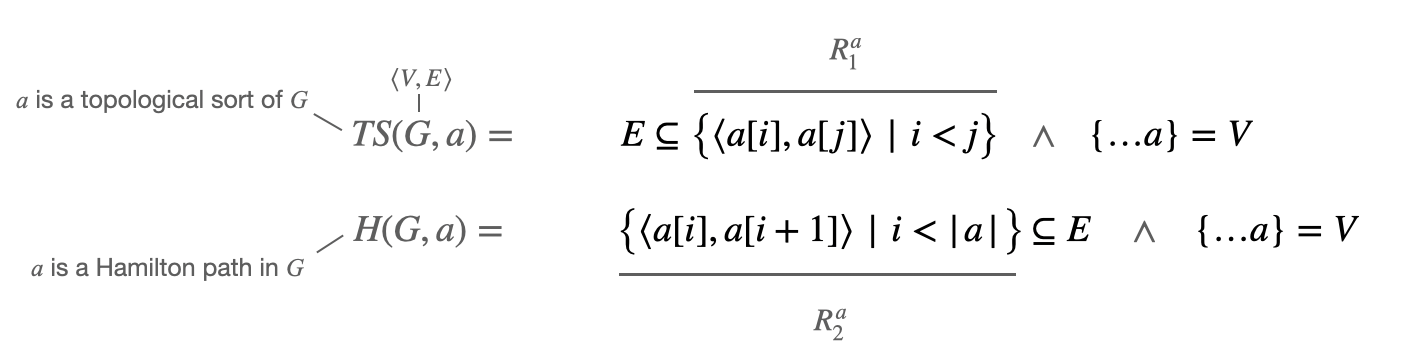
\includegraphics[width=.8\textwidth]{img/topological-and-hamilton.png}
\caption{Formal definitions of topological sort and Hamilton paths
  for use in \autoref{plan:hamilton}.}
\label{plan:hamilton-defs}
\end{figure}

I argue that the compact TC formulation allows for shorter proofs --- which, in turn, lead to easier proof derivation processes in both interactive and fully-automated settings.
We use the following example to illustrate this point; it is a problem taken from an undergraduate class on algorithms and complexity theory.

\begin{example}~\label{plan:hamilton}
\begin{tabular}[t]{lp{10cm}}
\textit{Given:} & A directed acyclic graph $G=\langle V,E\rangle$.
\\
\textit{Task:}  & Determine whether the graph contains a \emph{Hamilton path}; \ie, a (directed) path that visits every $u\in V$ exactly once.
\end{tabular}

\medskip
This exercise is given following a lecture on DFS, BFS, and topological sort.
This gives rise to the following short solution:
(1)~Topologically sort the vertices of $G$;
(2)~Check whether the resulting array constitutes a path,
 that is, every two consecutive elements are connected by an edge.
 
While the algorithm looks simple, it is not at all obvious that it is correct w.r.t.\@ the requirements.
Clearly, if step (2) returns $\ftrue$, then it has correctly discovered a Hamilton path (even without considering any properties of topological sort).
But when the outcome is $\ffalse$, some acute reasoning is required to show that there does not exist a \emph{different} ordering of $V$ that corresponds to a Hamilton path.
To establish correctness, the student needs to formalize the definition of topological sort and that of a Hamilton path
(\autoref{plan:hamilton-defs}).
Then the following proof goal must be accomplished:
\begin{equation}\label{plan:hamilton-goal}
\fH\,G\,a,~\fTS\,G\,a' ~\vdash~ a = a'
\end{equation}

That is, in a DAG containing a Hamilton path, there is exactly one possible topological sort, and that sort is identical to the order imposed by the Hamilton path.
(Notice that a DAG may contain at most one Hamilton path; this property is obtained as a simple corrollary of (\ref{plan:hamilton-goal}).)

An insight into the proof can be offered by considering the two binary relations $R_1^a$, $R_2^a$ occurring in the definitions of $\fTS$ and $\fH$.
A keen observer may notice that: $R_1^a = [{R_2^a}^+]$.
The implication would be that the topological sort ($R_1^a$) is uniquely determined by the Hamilton path ($R_2^a$) if the latter exists.
From there, proving (\ref{plan:hamilton-goal}) is by no means trivial, but it does follow from rather standard algebraic properties:
\begin{enumerate}
  \item $R_1^a$ is a \underline{\emph{total order}} on $V=\{...a\}$.
  \item A total order is \underline{\emph{maximal w.r.t.\@ set inclusion}}
    over all (partial) orders on the same set.
  \item The mapping $a \mapsto R_1^a$ is \underline{\emph{injective}}.
\end{enumerate}

Notably, the monotonicity of the transitive closure operator $^+$ (as of any closure operator) is utilized here to establish the relationship $R_1^a \subseteq R_1^{a'}$.
In this small instance, it is completely reasonable to expect that an automated prover can infer the three auxiliary properties listed above, as well as construct their proofs, without the user's intervention.
In more complex scenarios, the aspiration is toward the prover and the user working hand-in-hand, with the prover suggesting some conjectures that can progress the proof, and the user selecting the ones that make the most sense while also adding propositions that were not automatically discovered.
The use of algebraic concepts here is deliberate: the phrases ``total order'', ``set inclusion'', ``injective mapping'' all encode knowledge previously gained from human experience in defining and solving mathematical problems.
\end{example}

%\todo{describe the objective and how the transitive closure solver fits in the general scheme}

\begin{figure}
\begin{center}
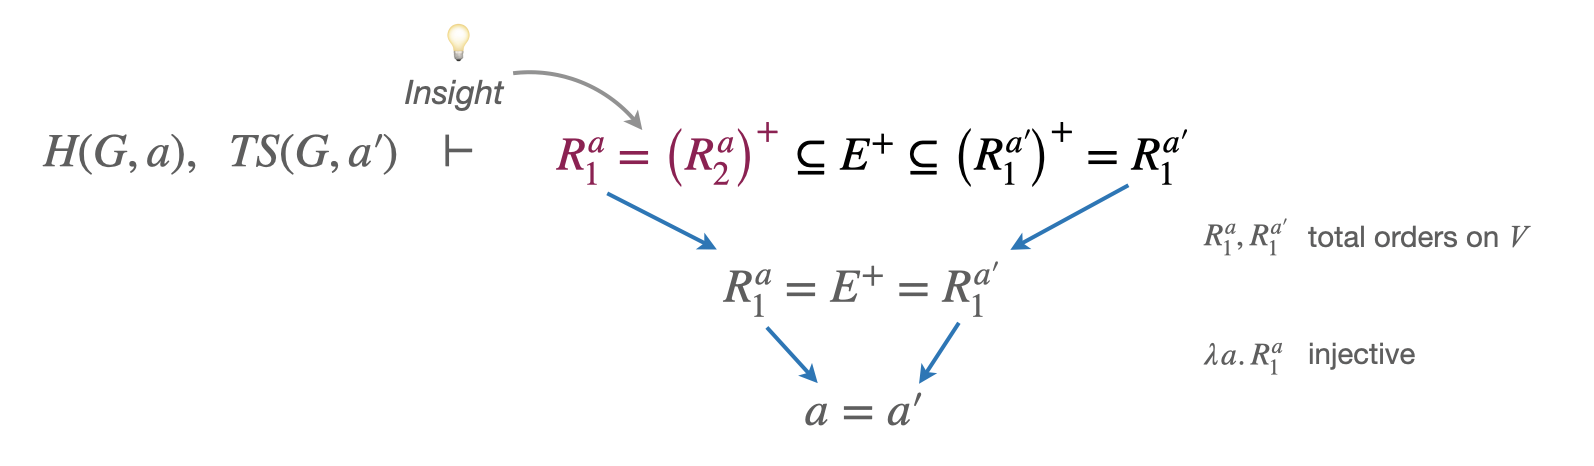
\includegraphics[width=.8\textwidth]{img/topological-and-hamilton-proof-sketch.png}
\end{center}
\vspace{-2em}
\caption{A sketch of the proof described in \autoref{plan:hamilton}.}
\label{plan:hamilton-proof}
\end{figure}


\begin{researchquestion}How can we leverage the success of cyclic proof systems for automated reasoning in TC (and co-TC)?
\end{researchquestion}

We would like to leverage the recent success of automated reasoning with cyclic proofs in Cyclist~\cite{CPP2017:Rowe}, and apply similar techniques to reasoning about properties encoded as TC formulas.
Cyclic systems for TC have been proposed~\cite{TOCL2020:Cohen,IJCAR2020:Cohen} and early experimentation with it (in a non-automatic setting) look very promising, as the proofs are elegant and large portions of them follow trivially by applying inference rules top-down, guided by the syntactic structure of the sub-goals.

It is of special interest to investigate if this guidance can be imporved by considering as a objective function the similarity between open sub-goals and their ancestors in the (partial) proof tree.
Bearing in mind that branches can be closed off by forming a cycle, processing a goal in a way that will allow it to be unified with an internal node (a companion) would be conducive to the overall proof effort.
In~\cite{PLDI2021:Itzhaky} my colleagues and I made use of the cyclic framework (for Separation Logic) for the purpose of improving state-of-the-art synthesis of pointer programs (\cite{POPL2019:Polikarpova}) by allowing the generation of auxiliary recursive functions.
These are extremely similar to ancillary lemmas whose proofs require induction, according to the proofs-as-programs correspondence, and this resonates well with our other objectives in \autoref{plan-modular}.

We also note that the proof rules shown in \autoref{b2:tc-cyclic} are biased, and correspond to a ``\emph{last step}''-oriented definition of RTC,
that is, the constructor grows a path by adding a step at the end:
%
\[\RTC{x,y}{\varphi}{s,t} ~~\Leftrightarrow~~
  s = t ~\lor~ \exists r.~\RTC{x,y}{\varphi}{s,r} \land \varphi[r,t]
\]
%
A dual definition is ``\emph{first step}''-oriented and adds a step at the beginning of the path instead:
%
\[\RTC{x,y}{\varphi}{s,t} ~~\Leftrightarrow~~
  s = t ~\lor~ \exists r.~\varphi[s,r] \land \RTC{x,y}{\varphi}{r,t}
\]

Although these definitions are very similar (and, of course, semantically equivalent), while experimenting with cyclic TC proofs we noticed that choosing one direction over the other can greatly simplify the proof.
When dealing with formulas having multiple occurrences of TC, it would become a crucial decision for automation which occurrence to apply the \rulename{TC$_{\textrm{L}}$}/\rulename{TC$_{\textrm{R}}$} rules to, and which variant of the rule to use.
This presents an opportunity to improve proof automation when compared to reasoning with general inductive definitions, where the freedom to choose the direction does not exist.

\begin{researchquestion}How can we combine inductive and deductive reasoning for automatic inference of proper induction hypotheses?
\end{researchquestion}

Deductive reasoning is the practice of applying general rules or statements to
individual, concrete cases; conversely, inductive reasoning is one of inferring,
from a set of observations, a unifying generalization.
Deductive reasoning can be thought of as a ``top-down'' application of logical
thinking, whereas inductive reasoning works ``bottom-up''.
While inferring a special case from a general case is always logically sound,
generalizing from examples can only guarantee soundness up to the set of
instances observed.
Still, even in the course of proving theorems, where soundness is of utmost
importance, humans habitually make use of inductive reasoning to guide their
deduction:
A handful of examples can give rise to a useful generalization, a lemma,
which can then be proven deductively.

ATPs employ deductive reasoning almost exclusively.
SMT solvers employ \emph{both} deductive reasoning (for example, propositional resolution) inductive reasoning in their inner workings.
Indeed, the latter are very much oriented toward constructing a model of the given formulas.
State-of-the-art SMT solvers make use of (partial) models generated in the
course of the search to guide deductive reasoning as this search progresses.
One notable example for this is Model-Based Quantifier Instantiation (MBQI)~\cite{CAV2009:Ge},
a technique implemented in Z3 to handle universally-quantified formulas.
In model checking, Counterexample-guided abstraction refinement (CEGAR)~\cite{ASPLOS2006:Solar-Lezama} is based on the notion of observing an abstract counterexample to guide predicate abstraction.
The most relevant works in the context of induction are those of invariant inference:
IC3 is heavily counterexample-guided, in that it makes progress by ``blocking'' states that are found to be unreachable.
Its ability to converge greatly depends on procedure for \emph{inductive generalization} that can draw stronger conclusions from the unreachability of a single state.
Without this generalization, IC3 will essentially have to enumerate all states, making it a very poor solution for symbolic model checking.
Similarly, ICE~\cite{CAV2014:Pranav} uses counterexamples, \esp counterexample-to-induction (CTIs), generalizing them to form candidate loop invariants.

Evidently, the idea of accumulating models of formulas or sub-formulas in the course of
a dialog between a deductive component and an inductive one can be lifted to
any type of reasoning.
What we wish to do in this research direction is to find the common core that makes the above work,
and how they can be integrated into automated reasoning tools proper.
When constructing proofs, existing models can be used to quickly vet possible
branching choices and discard ``obviously wrong'' ones: it is clearly futile
to try to prove a formula that is not valid, and any instance that does not
satisfy it can serve as a witness for that.
This is very much the process that a human mathematician may undergo when
considering which conjecture to prove next.
Clearly, having a representative set of models is essential for it, since
most intermediate statements have the form ``if $A_1$ and $A_2$ and $A_3$, then
$B$'', and models not satisfying one of the premises $A_i$ contribute no
relevant information.
It is thus desirable to identify ``pivot'' atomic formulas and keep around
models for various subsets of them.
\subsection{Modular Reasoning with Lemmas}
\label{plan-modular}

Mathematical proofs are seldom monolithic.
Usually, there are some intermediate conjectures --- \emph{lemmas} --- that
are proved one by one, gradually building toward the culmination of the main
theorem.
Mainly, it helps the author overcome the complexity of the proof development
task: in a formal setting, even a seemingly benign logical step can have many
inference steps; and the steps are not always sequential, for example when
a case split is required in order to consider several scenarios.
A hierarchical organization of tasks helps the author make sure that all the bases are covered, while not drowning in details.
This style of writing proofs has the additional benefit of making a proof easier to understand for potential readers.

There is much in common between this practice of organizing proofs and sub-proofs, and proven practices in software engineering.
In fact, the term \emph{proof engineering} has been coined recently~\cite{FTPL2019:Ringer} to drive this precise idea.
Like a programmer working on large systems, a scientist  developing complex proofs constructs abstractions, embodied in mathematical definitions, and then reasons about these abstractions at a high level, ignoring some concrete underlying details.
The scientist will prove properties about their abstractions as \emph{ancillary lemmas}, and then use these lemmas to derive desired properties.
What we intend to do in this research is to anchor this practice in support tools, and increase the level of automation by \textbf{automatically discovering and proving} these ancillary lemmas.

\begin{proposal}
Effective \emph{automatic} proof engineering requires a bidirectional approach, combining ``top-down'' reasoning --- decomposing top-level goals into smaller pieces,
and ``bottom-up'' reasoning --- constructing new conjectures that are consequences of known facts.
\end{proposal}

The core of this idea is in itself not new.
Starting from early theorem provers, the concept of \emph{information retention}~\cite{JAR1995:Voronkov} --- the derivation of new clauses by applying known inference rules and rewriting with equalities --- has been identified as an important feature for automated theorem proving, \esp when included in a prover that follows a top-down search strategy.
However, this proposal offers a new perspective on this aspect:
\begin{itemize}
  \item Where existing methods build consequences using small-step inference rules, we propose a paradigm that will make \textbf{larger logical leaps} by building on recent advances in lemma synthesis~\cite{CADE2013:Claessen,ITP2017:Johansson,arXiv2020:Singher,CAV2021:Murali} to create more useful lemmas that will hit the goals faster.
  \item We rethink the concept of \textbf{bottom-up through the lens of cyclic proofs}.
  Because the new systems admit infinite proofs~\cite{LICS2007:Brotherston,CPP2017:Rowe,IJCAR2020:Cohen}, they do not necessarily have a ``bottom'' in the traditional sense.
\end{itemize}

We allude to incremental construction of loop invariants presented in~\cite{arXiv2020:Padon,FAC2008:Bradley} as an inspiration for new, exciting ways to combine top-down and bottom-up search.


\begin{researchquestion}
What is an effective measure of \emph{usefulness} for ancillary lemmas, for the purpose of guiding theory exploration?
\end{researchquestion}

In~\cite{arXiv2020:Singher}, we explored an enumerative-synthesis approach to theory exploration with an emphasis on lemmas whose proofs require the use of induction.
A simple heuristic was used to choose lemmas that will be as generally applicable as possible.
This was sufficient for theorem proving benchmarks, but as the number of function symbols in the vocabulary grows, a more aggressive pruning will be necessary to avoid an unmanageable blowup in the number of lemmas.
We will develop an \textbf{a-priori clustering} of symbols from the vocabulary that are more tightly coupled, so that theory exploration can be applied to smaller vocabularies.
The clustering will be driven by the system's experience of proving theorems, which is accumulated over time, using statistical inference
This would mean that the prover will become more biased, but potentially much more effective, the more proofs it manages to successfully generate.
Even though we do not plan to use a deep-learning approach, a form of curriculum learning, where the system is exercised over a collection of problems with increasing complexity, will be used to bootstrap the prover's knowledge.

\begin{researchquestion}
What guidance metric would a prover use in order to \emph{untangle} a complex proof goal that mixes several mathematical concepts?
\end{researchquestion}

In order to make use of our lemmas, the vocabularies, that is, sets of logical symbols, occurring in propositions has to be clustered into ``tightly-coupled'' concepts.
Intuitively, functions or relations are tightly coupled if they occur together in ancillary lemmas; the more lemmas combine them, the more tightly coupled should they be considered.
This has practical implications:
If the prover manages to split the proof goal into sub-goals such that each sub-goal consists of tightly-coupled symbols, it will then have a larger variety of relevant lemmas to make progress with.
This \emph{untangle phase} can be multi-layered, since to get a separation into clusters A, B and C a prover may have to first separate A from B+C, and then separate B from C.
Each such separation is rarely a single derivation in the proof system, so some search, and backtracking, may be needed to nail down the right decomposition.
Here, too, I will apply statistical bias based on previous successful attempts at decomposing problems,
mimicking to a large degree the process of training an experienced mathematician.
\subsection{Extrapolating to Software}

As explained above, at the end of every software verification task there is a formal reasoning task, and that formal reasoning task is carried out solely at the level of the logical formula, paying no heed to the program for which the formula was generated.
In that sense, just building and improving a general-purpose automated prover is of immediate value to whatever verification tool is constructed on top of it.
However, there is one crucial pain point in reasoning about computer program, for which it is worth blurring the dichotomous boundary between code and logic.
This is the point of \textbf{representing program memory and memory updates}.

The first decade of the 21st century saw several breakthroughs in the analysis of programs with pointers and dynamic memory allocation.
Notably, \emph{Separation Logic}~\cite{LICS2002:Reynolds} was founded as a logic designed specifically for the purpose of modeling the heap area on which a program operates,
with dedicated inference rules in the style of Hoare to describe various effects on it.
Smallfoot~\cite{FMCO2005:Berdine} and GRASSHopper~\cite{TACAS2014:Piskac,CAV2014:Piskac} are examples of tools from that era, which can automatically prove propositions in Separation Logic.
At the same time, Shape Analysis based on Abstract Interpretation and 3-valued logic~\cite{CAV2014:Reps} became one of the most influential works in program analysis.
It is therefore surprising that state-of-the-art tools for automated software verification such as Dafny~\cite{LPAR2010:Leino}, VCC~\cite{vcc}, CIVL~\cite{civl}, and SeaHorn~\cite{CAV2015:Gurfinkel} \textbf{use none of that}.
The reason is, probably, the difficulty in using them within an SMT-based verifier, except in restricted cases
(\eg \cite{CAV2013:Piskac}).

At the same time, mechanical verification with \emph{interactive proof assistants} has skyrocketed in the last decade.
Thanks to their capacity to express higher-order propositions, Separation Logic has been embedded in Coq~\cite{PLDI2015:Sergey} and Isabelle/HOLCF~\cite{MFPS2008:Varming},
and substantial frameworks were erected for systematic treatment of unbounded-state programs with SL and it many variants.
Notable ones are VST~\cite{JAR2018:Cao}, Viper~\cite{VMCAI2016:Muller}, and Iris~\cite{POPL2015:Jung,ICFP2016:Jung,ESOP2017:Krebbers}, the latter becoming a cornerstone in recent years thanks to its ability to handle shared-memory concurrency in a variety of settings.
Some of the frameworks provide proof automation to a certain degree.
Thanks to the NSF's \emph{DeepSpec Expedition in Computer Science}, a plethora of formal verification success stories is now available in the form of proofs constructed by leading experts in the community.
This is a huge opportunity to harvest this corpus of knowledge and generalize from the hunderds of thousands of lines of Coq developments and other forms of proofs to drive our quest for more automation.
Being able to automate large classes of proofs that have been previously carried out in interactive proof assistants would be the culmination of my team's research.

\begin{proposal}
Instead of building provers that specialize in SL, we should strive to express the semantics of SL in our the logics that our provers support, thereby cultivating a healthier collaboration within the PL and Formal Methods community.
\end{proposal}

This is very much inspired by the success of SL in Coq as described above.
By providing tools like VST as libraries for Coq, the creators were able to tap into a vast pool of existing knowledge and experience.
I intend to repeat this successful strategy in the field of automated reasoning.
Doing so will require that we make some intermediate steps in which part of the reasoning would still be
\emph{user-guided} or \emph{supervised}.
The end goal remains to increase proof automation as much as possible.

\begin{researchquestion}
How can SL concepts be encoded in a logic based on TC,
and how can we use a generic TC prover (from \autoref{plan-induction})
to prove SL propositions?
\end{researchquestion}

This is an enticing question, because transitive closure can be used to define reachability properties,
and reachability has a dual meaning in program analysis: \emph{state reachability} refers to execution paths,
and \emph{heap reachability} refers to pointer paths in the program's memory.
I have explored this duality in~\cite{ESOP2021:Ish-Shalom},
where the concept was used to perfect safety proofs and complexity bound estimation.
State reachability is a standard notion corresponding to \textbf{induction over time};
heap reachability is used in Shape Analysis and is a form of \textbf{induction over space}.
Using the same mechanism to express both types of reachability allow for a uniform treatment of both kinds of induction, and opens the door to potential other kinds that can be harnessed.

\begin{figure}
\centering
\begin{tabular}{ll}
\begin{lstlisting}[basicstyle=\linespread{1.36}\ttfamily\fontsize{10pt}{8pt}\selectfont]
reverse(h) :=
  i := h;
  j := null;
  while (i != null) {
    t := i.next;
    i.next := j;
    j := i;
    i := t;
  }
\end{lstlisting}
&
\def\hdist{3mm}
\def\hdistnul{1mm}
\def\vdist{4mm}
\def\vdistptr{1.1mm}
\def\vdistptrj{0.8mm}

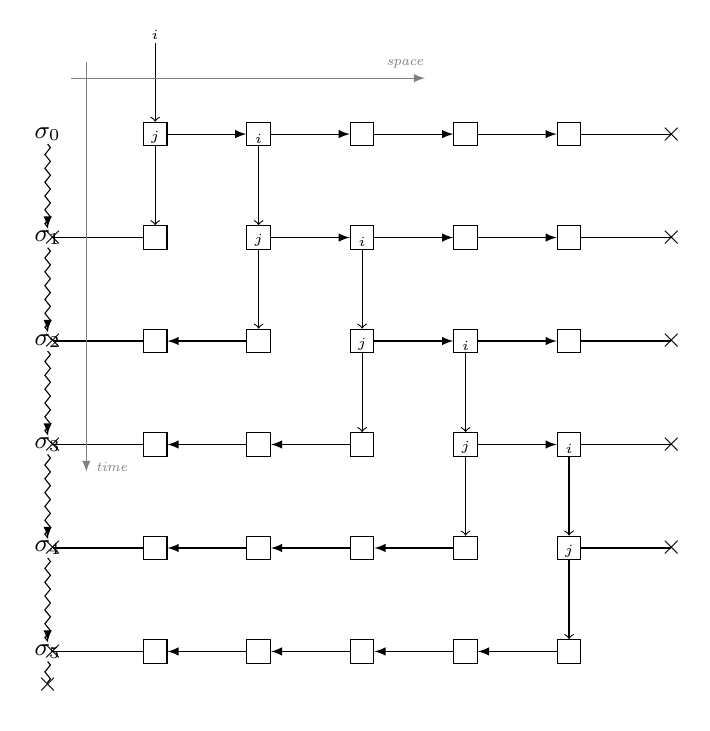
\begin{tikzpicture}[link/.style={draw, minimum size=3mm}, baseline={(current bounding box.center)},
    state/.style={font=\small, inner sep=1pt},
	ptr/.style={font=\tiny, inner sep=1pt},
    buzz/.style={decorate,
      decoration={zigzag, amplitude=1pt,
      segment length=5pt}}]
    
  \node(s1u0)[link] {};
  \node(s1u1)[link, right=\hdist of s1u0] {};
  \node(s1u2)[link, right=\hdist of s1u1] {};
  \node(s1u3)[link, right=\hdist of s1u2] {};
  \node(s1u4)[link, right=\hdist of s1u3] {};
  \node(s1nul)[right=\hdistnul of s1u4, inner sep=0] {$\times$};
  \draw[-latex] (s1u0) -- (s1u1);
  \draw[-latex] (s1u1) -- (s1u2);
  \draw[-latex] (s1u2) -- (s1u3);
  \draw[-latex] (s1u3) -- (s1u4);
  \draw (s1u4) -- (s1nul.center);
  \node(s1i)[ptr, above=\vdistptr of s1u0]{$i$};
  \draw[->] (s1i) -- (s1u0);
  
  \node(s0)[state, left=of s1u0] {$\sigma_0$};
  
  %
  
  \node(s2u0)[link, below=\vdist of s1u0] {};
  \node(s2u1)[link, right=\hdist of s2u0] {};
  \node(s2u2)[link, right=\hdist of s2u1] {};
  \node(s2u3)[link, right=\hdist of s2u2] {};
  \node(s2u4)[link, right=\hdist of s2u3] {};
  \node(s2nul)[right=\hdistnul of s2u4, inner sep=0] {$\times$};
  \node(s2bk)[left=\hdistnul of s2u0, inner sep=0] {$\times$};
  \draw (s2u0) -- (s2bk.center);
  \draw[-latex] (s2u1) -- (s2u2);
  \draw[-latex] (s2u2) -- (s2u3);
  \draw[-latex] (s2u3) -- (s2u4);
  \draw (s2u4) -- (s2nul.center);
  \node(s2i)[ptr, above=\vdistptr of s2u1]{$i$};
  \draw[->] (s2i) -- (s2u1);
  \node(s2j)[ptr, above=\vdistptrj of s2u0]{$j$};
  \draw[->] (s2j) -- (s2u0);

  \node(s1)[state, left=of s2u0] {$\sigma_1$};
  
  %
  
  \node(s2u0)[link, below=\vdist of s2u0] {};
  \node(s2u1)[link, right=\hdist of s2u0] {};
  \node(s2u2)[link, right=\hdist of s2u1] {};
  \node(s2u3)[link, right=\hdist of s2u2] {};
  \node(s2u4)[link, right=\hdist of s2u3] {};
  \node(s2nul)[right=\hdistnul of s2u4, inner sep=0] {$\times$};
  \node(s2bk)[left=\hdistnul of s2u0, inner sep=0] {$\times$};
  \draw (s2u0) -- (s2bk.center);
  \draw[-latex] (s2u1) -- (s2u0);
  \draw[-latex] (s2u2) -- (s2u3);
  \draw[-latex] (s2u3) -- (s2u4);
  \draw (s2u4) -- (s2nul.center);
  \node(s2i)[ptr, above=\vdistptr of s2u2]{$i$};
  \draw[->] (s2i) -- (s2u2);
  \node(s2j)[ptr, above=\vdistptrj of s2u1]{$j$};
  \draw[->] (s2j) -- (s2u1);
  
  \node(s2)[state, left=of s2u0] {$\sigma_2$};
  
  %
  
  \node(s2u0)[link, below=\vdist of s2u0] {};
  \node(s2u1)[link, right=\hdist of s2u0] {};
  \node(s2u2)[link, right=\hdist of s2u1] {};
  \node(s2u3)[link, right=\hdist of s2u2] {};
  \node(s2u4)[link, right=\hdist of s2u3] {};
  \node(s2nul)[right=\hdistnul of s2u4, inner sep=0] {$\times$};
  \node(s2bk)[left=\hdistnul of s2u0, inner sep=0] {$\times$};
  \draw (s2u0) -- (s2bk.center);
  \draw[-latex] (s2u1) -- (s2u0);
  \draw[-latex] (s2u2) -- (s2u1);
  \draw[-latex] (s2u3) -- (s2u4);
  \draw (s2u4) -- (s2nul.center);
  \node(s2i)[ptr, above=\vdistptr of s2u3]{$i$};
  \draw[->] (s2i) -- (s2u3);
  \node(s2j)[ptr, above=\vdistptrj of s2u2]{$j$};
  \draw[->] (s2j) -- (s2u2);

  \node(s3)[state, left=of s2u0] {$\sigma_3$};
  
  %
  
  \node(s2u0)[link, below=\vdist of s2u0] {};
  \node(s2u1)[link, right=\hdist of s2u0] {};
  \node(s2u2)[link, right=\hdist of s2u1] {};
  \node(s2u3)[link, right=\hdist of s2u2] {};
  \node(s2u4)[link, right=\hdist of s2u3] {};
  \node(s2nul)[right=\hdistnul of s2u4, inner sep=0] {$\times$};
  \node(s2bk)[left=\hdistnul of s2u0, inner sep=0] {$\times$};
  \draw (s2u0) -- (s2bk.center);
  \draw[-latex] (s2u1) -- (s2u0);
  \draw[-latex] (s2u2) -- (s2u1);
  \draw[-latex] (s2u3) -- (s2u2);
  \draw (s2u4) -- (s2nul.center);
  \node(s2i)[ptr, above=\vdistptr of s2u4]{$i$};
  \draw[->] (s2i) -- (s2u4);
  \node(s2j)[ptr, above=\vdistptrj of s2u3]{$j$};
  \draw[->] (s2j) -- (s2u3);

  \node(s4)[state, left=of s2u0] {$\sigma_4$};
  
  %
  
  \node(s2u0)[link, below=\vdist of s2u0] {};
  \node(s2u1)[link, right=\hdist of s2u0] {};
  \node(s2u2)[link, right=\hdist of s2u1] {};
  \node(s2u3)[link, right=\hdist of s2u2] {};
  \node(s2u4)[link, right=\hdist of s2u3] {};
  \node(s2bk)[left=\hdistnul of s2u0, inner sep=0] {$\times$};
  \draw (s2u0) -- (s2bk.center);
  \draw[-latex] (s2u1) -- (s2u0);
  \draw[-latex] (s2u2) -- (s2u1);
  \draw[-latex] (s2u3) -- (s2u2);
  \draw[-latex] (s2u4) -- (s2u3);
  \node(s2j)[ptr, above=\vdistptrj of s2u4]{$j$};
  \draw[->] (s2j) -- (s2u4);

  \node(s5)[state, left=of s2u0] {$\sigma_5$};

  %
  
  \node(exit)[below=.5mm of s5] {$\times$};
  
  \draw[buzz, -latex] (s0) -- (s1);
  \draw[buzz, -latex] (s1) -- (s2);
  \draw[buzz, -latex] (s2) -- (s3);
  \draw[buzz, -latex] (s3) -- (s4);
  \draw[buzz, -latex] (s4) -- (s5);
  \draw[buzz] (s5) -- (exit.center);
  
  \node(origin)[above right=4mm of s0, yshift=3mm, coordinate] {};
  \node(time)[below=50mm of origin, coordinate] {};
  \draw[gray,-latex] (origin) -- (time) node[right,anchor=south west, inner ysep=0] {\tiny\textit{time}};

  \node(space)[right=43mm of origin, coordinate] {};
  \draw[gray,-latex] (origin) -- (space) node[right,anchor=south east, inner xsep=0] {\tiny\textit{space}};
  
  \draw[gray] (origin) -- +(-2mm,0);
  \draw[gray] (origin) -- +(0,2mm);

\end{tikzpicture}
\end{tabular}
\caption{A program that reverses a linked list in-place;
 a canonical example from~\cite{LICS2002:Reynolds}.
 Notice the isomorphism between the time and the space axes.
 }
\label{b2:software-reverse}
\end{figure}

Notice how in the example program \texttt{reverse}
of \autoref{b2:software-reverse},
the duality between the \emph{time} axis (successive states in the execution trace) and the \emph{space}
axis (links in the singly-linked list, \esp those pointed to by $i$ and $j$).
The end of the list, denoted by a null pointer,
corresponds to the exit state.

\smallskip
After having obtained a suitable solution for modeling program memory in our automated reasoning,
we set as a goal to automate challenging objectives from the DeepSpec expedition code base.
These serve triple purpose:
\begin{enumerate}
  \item As evaluation milestones for self-check and monitoring the project's progress.
  \item As a driving force for the identification of interesting theoretical and practical problems and the pursuit of appropriate solutions.
  \item As a means to disseminate our results and bring forth its adoption by the larger formal methods community, since DeepSpec is famous for being a grand undertaking.
\end{enumerate}

The remainder of this objective therefore comprised not of research questions but as a sequence of ongoing experimental setups where the team strives to cover ground in DeepSpec, \esp the following components and their associated proofs:
\begin{enumerate}
  \item CertiKOS: certified OS kernel.
  \item DataCert: DBMS and SQL service.
  \item CompCert: certified C compiler.
  \item Galois: electronic voting system with strong guarantees against fraud.
\end{enumerate}



\clearpage
\hrule
\section{Research Plan \todo{B2}}

\subsection{Inductive-Deductive Reasoning Hybrid}

Deductive reasoning is the practice of applying general rules or statements to
individual, concrete cases; conversely, inductive reasoning is one of inferring,
from a set of observations, a unifying generalization.
Deductive reasoning can be thought of as a ``top-down'' application of logical
thinking, whereas inductive reasoning works ``bottom-up''.
While inferring a special case from a general case is always logically sound,
generalizing from examples can only guarantee soundness up to the set of
instances observed.
Still, even in the course of proving theorems, where soundness is of utmost
importance, humans habitually make use of inductive reasoning to guide their
deduction:
just a handful of examples can give rise to a useful generalization, a lemma,
which can then be proven deductively.

While there is no perfect analogue in the prover/solver setting as portrayed
in \autoref{intro}, it is quite obvious that theorem provers employ deductive
reasoning almost exclusively.
It would be inaccurate to say that SMT solvers employ inductive reasoning in
the same sense; a lot of their mechanics is still based on deduction.
However, they are very much oriented toward constructing a model of the given formulas.
State-of-the-art SMT solvers make use of (partial) models generated in the
course of the search to guide deductive reasoning as this search progresses.
One notable example for this is Model-Based Quantifier Instantiation (MBQI),
a technique implemented in Z3.
In Sketch, a software synthesis tool, the system observes a set of inputs (and
outputs), proposes a generalization (a program), and then attempts to verify it
using a deductive method (in their case, reduction to SAT).\todo{what no, need to explain the use of counterexamples}
A growing number of examples is needed for the generalization to yield a correct
program, so this process repeats in a loop.

The idea of accumulating models of formulas or sub-formulas in the course of
a dialog between a deductive component and an inductive one can be lifted to
any type of reasoning.
When constructing proofs, existing models can be used to quickly vet possible
branching choices and discard ``obviously wrong'' ones: it is clearly futile
to try to prove a formula that is not valid, and any instance that does not
satisfy it can serve as a witness for that.
This is very much the process that a human mathematician may undergo when
considering which conjecture to prove next.
Clearly, having a representative set of models is essential for it, since
most intermediate statements have the form ``if $A_1$ and $A_2$ and $A_3$, then
$B$'', and models not satisfying one of the premises $A_i$ contribute no
relevant information.
It is thus desirable to identify ``pivot'' atomic formulas and keep around
models for various subsets of them.






\subsubsection{Using Implicit Induction}

Most theorem provers, as well as some SMT solvers and systems using them,
prove inductive properties by the introduction of an \emph{induction scheme} ---
a specialized inference rule, whose premises comprise the induction base case
and step.
For example, given $P(0)$ and $\forall k.~ P(k)\rightarrow P(k+1)$,
one can infer $P(n)$ for any natural $n$.
In this way, the induction step effectively ``hides'' several application of
the induction hypothesis $P(k)$ inside a single inference step.
This is much different from the way humans approach the problem: they may set
out simplifying $P(k)$, realizing at some point that it may follow from $P(k-1)$,
justifying such reasoning based on the natural numbers being a wellfounded set.

\todo{this is the completely wrong setup. it has been shown to be effective already, it is no longer a conjecture.}
{\color{gray}We conjecture that this \emph{implicit} induction approach is suitable for
automatic proof discovery as well.
The formal implementation in this context is that of \emph{cyclic proof systems};
the cyclic framework admits proofs where some premises are satisfied by
conjectures occurring \emph{later} in the goal.
Of course, for such proofs to be sound some side conditions are imposed to assure
that a wellfounded order can be established.
}

\subsubsection{Overcome the Frame Problem with Frame Properties}

A prevalent difficulty of reasoning in logic is the \emph{frame problem}:
a constant need to specify not only effects we are interested to reason about,
but the entire environment surrounding it, which was not directly affected.
In the context of reasoning about computer systems, a program may effect a change
by storing or removing some data, causing a change in the system's state.
In order to prove properties of the system, and in particular, of such
accumulated changes, logic dictates that we formulate precisely what has
\emph{not} change in the system's state, including memory locations, database
tables, network communication packets \etc, that the program did not touch.
This is a huge hinderance to effective reasoning since properties that were
assumed or already proven with regard to the input state, have to be
re-stated and proven respective to the new state.
Such proofs are mundane and daunting, but there are many such properties
popping up in the course of a proof and they may very well require more work to
discharge than the ``insightful'' part.

\begin{figure} 
\begin{lstlisting}[basicstyle=\linespread{1.36}\ttfamily\fontsize{10pt}{8pt}\selectfont]
reverse(h) :=
  i := h; j := null;
  while (i != null) {
    t := i.next;
    i.next := j; j := i;
    i := t;
  }
\end{lstlisting}
\end{figure}

A classical example for the severity of the problem is analysis of the program
\textsf{reverse}, which reverses the order of nodes in a singly-linked list.
The program flips one edge at a time, and the effect of each iteration is
very local; however, to prove even a most basic property, that the program does
not introduce cycles in the list, the programmer has to include properties of
the prefix and suffix of the list, which have not changed --- the ``frame''.
The bookkeeping difficulty was so intense, that it led John C. Reynolds to the
conclusion that reasoning about pointer paths using transitive closure (heap
reachability) is not practical, and to found a new logic for dealing with
programs with dynamic heaps.
This logic is known as Separation Logic and is still the state-of-the-art in
reasoning about heaps.

%\begin{figure}
%\includegraphics[width=5cm]{standalone}
%\embedlatex[width=5cm]{standalone}
%\end{figure}

We claim that transitive closure \emph{can} be made effective by harnessing
\emph{frame properties} arising from the theory of transitive closure.
Frame properties are theorems and lemmas that assert the preservation of
certain properties, across consecutive program states, subject to the more
fine-grained properties preserved by the transition between them.
Frame properties can be generic or specific; \emph{generic} frame properties are
schemas that can apply to any $\varphi$ formula occurring within a transitive
closure $\big(\mathrm{TC}_{x,y}\varphi\big)$.
\emph{Specific} frame properties pertain to concrete programs and their respective
state transition semantics expressed as formulas.
An example of a generic property is: if there is a $\varphi$-path between some
two individuals $u, v$, and if for any $x,y$ $\varphi$-reachable from $u$, it
holds that $\varphi(x,y) \leftrightarrow \psi(x,y)$, then there is also a
$\psi$-path between $u, v$.
A derived, specific frame property could be the following: assume $n$ is a
function symbol representing the pointer links of a linked list, and assume
$n'$ is another function symbol representing the links of the same list after
a \emph{single iteration} of the program \textsf{reverse}.
Then all nodes reachable from the \emph{successor} of the loop iterator in the
former list, are still reachable from it in the second list.
This follows from the fact that the location of the modified pointer is not
reachable from any of the nodes in question, so the link paths in that area of
the list (the suffix) could not be affected.

\todo{example for frame property(-ies) in TC}

\begin{figure}
\centering
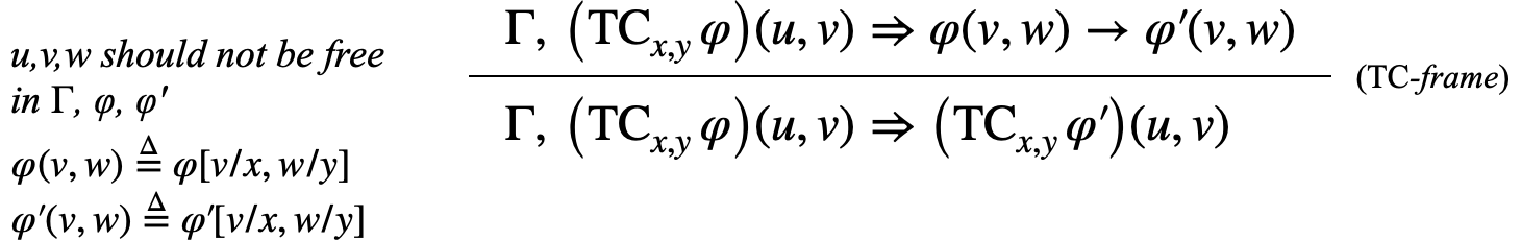
\includegraphics[width=10cm]{img/tc-frame-gen.pdf}
\caption{Generic frame property for (reflexive) TC}
\end{figure}

By developing proof-support tools that ``guess'' specific frame properties
% xref lemma speculation
and prove them automatically based on more primitive facts and by applying
generic frame properties, we expect to greatly improve the efficacy of theorem
provers and also of interactive proof assistants in handling conjectures
involving transitive closure.
While frame properties do not, formally, play any special role compared to
other formulas occurring throughout the proof, they follow a unique kind of
``thought pattern'' that serves a mental purpose in abstracting away nitpicky
details.
This would allow us to focus human and machine attention alike on the more
nitty-gritty parts of the proof.

\subsubsection{Next-level Transitive Closure}

The use of transitive closure logic is not restricted to reasoning about heap
graphs, which mostly involved low-level kind of reasoning.
Many aspects of computing rely on iteration, \eg when expressing properties of
aggregate data --- a sum of a column in a database, for instance.
Indeed, there is a large and interesting space of programs that can be realized
with the combination of the functional operations \textsf{map}, \textsf{filter},
and \textsf{reduce}. % cite SPARK
Sets and sequences can be stored in many ways in memory and in non-volatile
storage, yet the iteration aspect remains the same and can be characterized by
a ``next-in-iteration'' function that matches for each element, the following
element in the iteration order.
The loopy construct, \eg sum, can then be axiomatized using the transitive
closure $\big(TC_{\langle a,u\rangle,\langle b,v\rangle}v=n(u) \land b=a+\mathrm{val}(u)\big)$
With the help of TC support in the theorem prover, and in the presence of a
library of theorems defining known properties of TC, reasoning about such
aggregates can be streamlined to be simpler than by using the corresponding
inductive definition of sum.
For example, distributivity of sum over sequence concatenation follows (almost)
for free from the transitivity of TC.



\subsection{Modular Reasoning with Lemmas}

Mathematical proofs are seldom monolithic.
Usually, there are some intermediate conjectures --- \emph{lemmas} --- that
are proved one by one, gradually building toward the culmination of the main
theorem.
It is not done out of altruism towards potential readers of the paper, though it can
certainly make a proof easier to understand.
Mainly, it helps the author overcome the complexity of the proof development
task: in a formal setting, even a seemingly benign logical step can have many
inference steps; and the steps are not always sequential, for example when
a case split is required in order to consider several scenarios.

This kind of modularization has been carried over by computer scientists to the
realm of interactive proof assistants.
In Type Theory, the use of lemmas is wired in as they are reduced to function
calls following the Curry-Howard Correspondence.
Modular proofs are even more of the essence in automated proof search, due to
the inherent computational complexity of the tool and poor scalability of
existing search techniques.
Breaking a proof task into lemmas also carries the promise of combining different
approaches to finding the proofs, by applying a portfolio approach in the spirit
of Why3 \cite{}.

\subsubsection{...}

\subsubsection{Near-match Lemma Speculation}

The following is a common scenario for anyone who has worked on formal proof development:
you have a conjecture to prove, and there is
a theorem whose conclusion seems to fit the conjecture, but does not \emph{quite} match.
As a very simple example, suppose the conjecture is
$\exists k.~ n = 2\cdot k$, and the preexisting theorem states:
\begin{equation}\label{manna-divmod}
  \forall i, j.~ i = \fdiv(i, j) \cdot j + \frem(i, j)
\end{equation}

(Inspired by Manna and Waldinger, 1980.)
Strict syntactic unification would fail to apply (\ref{manna-divmod}) to the proof goal $n = 2\cdot \evar{k}$, since (\ref{manna-divmod}) has a $+$ operator on the right-hand side of the equality.
(Here and in the sequel, we use $\evar{k}$ to designate a pattern variable that can be unified with anything.)
However, an intelligent mathematician knows that according to the basic laws of arithmetic, $\forall x.~x + 0 = x$.
It is possible to ``unblock'' the unification process if we equate $\frem(\cdot,\cdot) = 0$.
Similarly, unifying $\fdiv(n,\evar{j})\cdot \evar{j}$ with $2\cdot \evar{k}$ would fail, since $2$ cannot be unified with $\fdiv(n,\evar{j})$.
Again, by the law of commutativity, 
$\fdiv(n,\evar{j})\cdot j = \evar{j} \cdot\fdiv(n,\evar{j})$,
so we should be able to unify $\evar{j}$ with $2$ and $\fdiv(n, 2)$ with $\evar{k}$.

This process of \emph{unification modulo equalities}, or \emph{E-unification}, has been explored in the past but never exploited for automation\citeneeded{}.

{\color{gray}
transitive closure (see above) of a unary function $n$.
Transitivity dictates that this follows from $n^*(x,v), n^*(v,z)$ for some $v$,
and there is an assumption, or a previously proven conjecture, $n^*(x,y)$;
however, no assumption $n^*(y,z)$ is available.
Instead, what you have is $m^*(y,z)$ for a second function $m$.
This can be overcome by proving that $m^*(y,z) \Rightarrow n^*(y,z)$, as a
separate lemma.
To prove such a lemma, one may try to prove that $n=m$, or that $n^*=m^*$,
or that $\forall u, n^*(y,u)\leftrightarrow m^*(y,u)$, or any other generalization
of the missing implication.}

To mechanize the process, a prover is required to select a suitable version.
Some alternatives can be vetted out using the model-based approach described
earlier.
Proving the auxiliary lemma can also be postponed to a later stage, after the
prover has concluded the current proof branch and admitted it --- since a failed
proof branch will be discarded anyway, and all the lemmas used in it become
moot.
Hence the term ``speculation'', also used in works on proofs by rippling \cite{}.
In the original presentation, speculated lemmas are equalities between terms,
but they can be made far more general and integrate
into any kind of clause-based inference system such as natural deduction or
sequent calculus used by modern provers.


\subsubsection{Semi-eager Theory Propagation}

The T of SMT stands for \emph{Theory}.
A theory in this context comprises of a specific vocabulary, inducing a limited
subset of logical formulas, and a designated interpretation, thus also limiting
the logical \emph{structures} that can be considered for them.
One popular example, built into many SMT solvers, is the theory of integer linear
arithmetic (LIA): it provides the operators ``$+$'', ``$-$'', ``$\cdot$'' as
well as order relations ``$=$'', ``$\leq$''.
It imposes a syntactic restriction that two variables may not be multiplied;
a variable may only be multiplied by a constant numeric literal.
While a formula such as $5 < 3$ is \emph{logically} satisfiable, it is
unsatisfiable in the theory of LIA, since it requires all numeric literals to
be interpreted as the integers they represent and that ``$<$'' be interpreted
as the order of integers.

Communication between the SAT component and the theory component of the model
is handled by the theory solver producing \emph{learned clauses} that are valid
modulo the theory and a logically unsatisfiable when conjoined with the existing
goal.
For $5 < 3$, this may be as simple as $\lnot(5 < 3)$; but the clauses get more
involved as problem sizes and number of variables grow.
The generation of clauses by the theory solver is called
\emph{theory propagation}, and can be done in two ways: (i) \emph{eagerly}, by
observing the formula given to the solver and generating all the theory-valid
statements containing the terms it contains; and (ii) \emph{lazily}, waiting for
SAT to produce a Boolean assignment and then contradicting it with
appropriate clauses when it is inconsistent with the theory.

The eager approach has an inherent flaw: the number of such theory-valid
statements can grow very large very quickly.
It can be infinite, in the case of some theories, as most theories are
represented, conceptually speaking, by quantified formulas, and there is no
bound on the number of instantiations that may be needed to refute a single
statement.
Some theories, in particular those of integers, are not even definable by any
finite set of first-order formulas, quantified or otherwise.
Such difficulties cause eager propagation techniques to be all but abandoned.

The lazy approach, despite its popularity, can have severe run-time
implications.
It means that a number of SAT assignments have to be observed, and a
potentially computation intensive procedure consulted, to refute their
satisfiability in the logic.
Designers of SMT try to be clever in the way propagation clauses are generated,
since generating more general clauses will drive the SAT away from more
inconsistent assignments at an earlier stage, saving calls to theory solver.
This tactic is limited, however, since the theory solver only gets a glimpse
of a narrow case each time it is involved, and cannot make global decisions
based on the structure of the entire input problem.

We propose a middle ground, and that middle ground involves a more holistic view of the proofs.
In a combined setting where SAT, theories, and formal proof objects work
together, intermediate proofs being explored provide ample subformulas to
fertilize propagation.
We will define an \emph{integration metric} for propagation clauses, that
quantitively expresses how tightly coupled a potential clause is with the
existing set of assumptions and goals present in the proof.
This can be thought of as a miniature ``page rank'' for logical formulas:
``hot'' atomic formulas, that is, ones that occur often in the proof, encourage
clauses that contain them, and these clauses, if accepted, will light up
more atomic formulas, with rank diminishing as they drift further from the
core.
Then, we will construct effective algorithms for finding such clauses that
optimize this metric.
We will tune the metric and the algorithms to achieve the fastest convergence
and compare to existing heuristics.

This semi-eager propagation of clauses from theories hold true potential for
a breakthrough with respect to handling theories and quantified conjectures
in unison, as challenged by Voronkov \citeneeded{}.


\subsubsection{Lemma Patching}

Again, this is inspired by the way mathematicians work, first proving a
simplified version of a desired property as a lemma, then inspecting the proof
to figure out ``what would go wrong'' in the more general case --- using that to guide insight toward
proving a stronger lemma.
Intermediate proofs are thus raw material for more proofs: this lends a
``white-box'' view of lemmas, complementing the more basic use of lemmas in
their closed form, encapsulating their proofs (which can be seen as
``black-box'').
In a dual manner, occasionally a lemma is too strong: \eg, if its conclusion is
a conjunction, but one is only interested in one of the conjuncts.
It is possible that a subset of the premises is sufficient to prove that one
conjunct.
Another example is when a conclusion is of the form $a < b$, but a relaxed set
of premises is enough to obtain $a \leq b$.

Moreover, during proof exploration itself (either by human or by machine), some
incorrect, dead-end proofs are inevitably encountered.
These are characterized, indeed identified, by assumptions that cannot be made
soundly (\eg a proof branch that includes formulas that are not logically valid).
Normally, a theorem prover simply discards these failed attempts and tries
other directions.
However, these too can be leveraged as raw material; repairing them amounts to
eliminating the spurious, invalid assumptions.

\begin{figure}
\centering
\raisebox{-.33\height}{
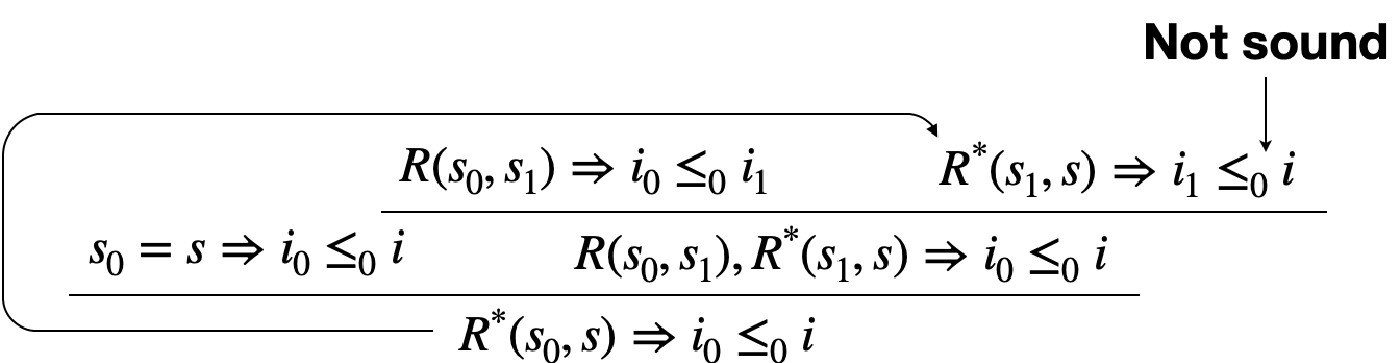
\includegraphics[width=7cm]{img/lemma-patching.pdf}}
$\longrightarrow$~~
\raisebox{-.33\height}{
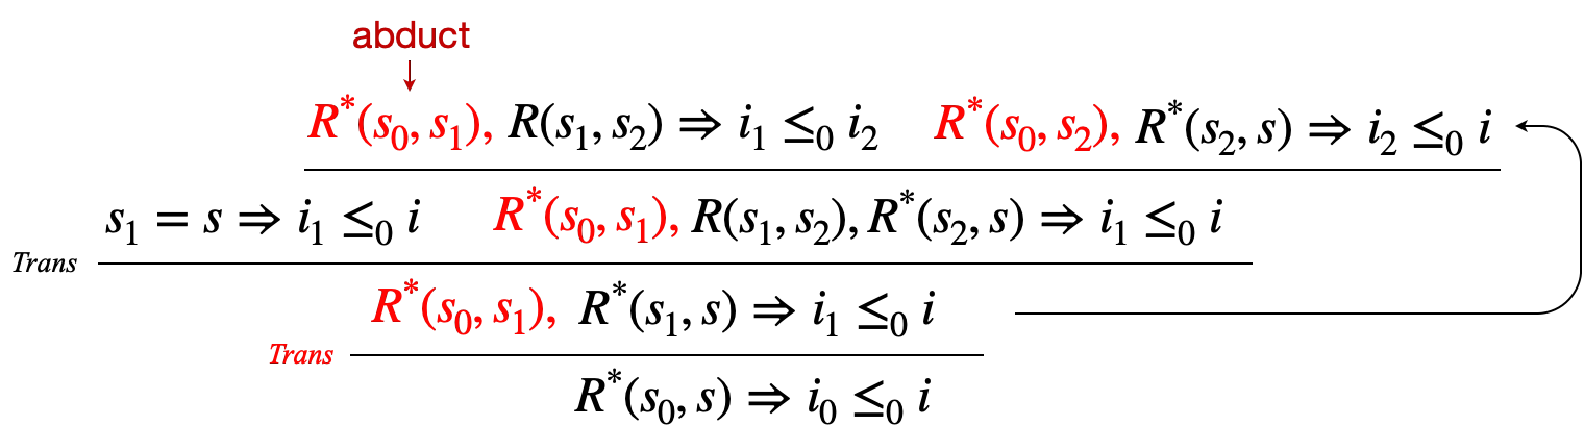
\includegraphics[width=7.5cm]{img/lemma-patching-abduct.pdf}
}
\caption{Example for lemma patching}
\label{lemma-patching-example}
\end{figure}

\todo{refer to \autoref{lemma-patching-example}}


\subsection{Extraploating to Software}

As much as mechanical theorem proving is useful for formalizing mathematics, it has much wider and more exciting uses when it comes to reasoning about computer programs and their semantics.
To date, the most popular text on interactive theorem proving in Coq is the Software Foundations series~\citeneeded{}, a collaborative community
effort to formalize programming language concepts
and verification problems.
The example proofs and exercises in the textbook make some use of proof automation facilities existing in Coq.
These are, however, far from what can be offerred by dedicated automated provers and solvers.
This research aspires to bring such automated tools to a new level, in which they will be able to cope with these fundamental tasks naturally and directly.
Most importantly, that they will be capable of handling such formal definitions as occur in~\citeneeded{(SF again)} naturally, without requiring the user to translate their claims into a restricted logical fragment.

\subsubsection{Homotopy for Programs}

Homotopy Type Theory~\citeneeded{} is an emerging field of study offering a fresh view on Martin-L\"of  Type Thoery, in which type judgements are given
first-class-citizen status.
Types can be declared isomorphic, allowing terms of one type to be interpreted as the other type.
In the field of mathematics, homotopy is quite valuable, since it enables the transfer of knowledge (definitions and theorems) across related fields.
We claim an insight, that homotopy is predominant in software as well.
As such, it can be leveraged to many automated reasoning tasks revolving around computer programs.
We point out two situation in which homotopy arises naturally in programming.

\begin{paragraph}{Alternative representations}
Oftentimes, the same data can be described in more than one way.
This can arise from a discrepency between libraries, or an abstraction gap between specification and implementation levels.
\end{paragraph}

\bibliographystyle{plain} 
\bibliography{bib}

\end{document}

